\documentclass[11pt,a4paper]{article}

\usepackage[margin=0.82in]{geometry}
\usepackage{mathptmx}
\usepackage{graphicx}
\usepackage{booktabs}
\usepackage{float}
\usepackage{subcaption}
\usepackage{caption}
\usepackage{setspace}
\usepackage{titlesec}
\usepackage{microtype}
\usepackage{amsmath}
\usepackage{array}
\usepackage{placeins}
\usepackage[numbers,sort&compress]{natbib}
\usepackage[colorlinks=true,linkcolor=black,citecolor=black,urlcolor=blue]{hyperref}

\graphicspath{
  {./}
  {../results/trajectory_analysis/figures/}
  {../results/GSE150318/figures/}
  {../results/GSE79396_tPCA/figures/}
  {../results/GSE79396_response/figures/}
}

\captionsetup{font=footnotesize,labelfont=bf,skip=3pt}
\setstretch{1.0}
\setlength{\parindent}{1.25em}
\setlength{\parskip}{0pt}
\setlength{\emergencystretch}{2em}
\setlength{\textfloatsep}{7pt plus 1pt minus 2pt}
\setlength{\floatsep}{6pt plus 1pt minus 1pt}
\setlength{\intextsep}{6pt plus 1pt minus 1pt}
\setlength{\abovecaptionskip}{3pt}
\setlength{\belowcaptionskip}{0pt}
\setlength{\tabcolsep}{4pt}
\renewcommand{\arraystretch}{0.92}
\titlespacing*{\section}{0pt}{1.1ex plus .2ex}{0.6ex}
\titlespacing*{\subsection}{0pt}{0.9ex plus .2ex}{0.4ex}

\title{\textbf{Trajectory-aware transcriptomic analysis of aging and vaccine-response datasets with tensorOmics}}
\author{Zilong Wang}
\date{Internship report, 2026}

\begin{document}

\begin{titlepage}
  \centering
  \vspace*{2cm}
  {\Large Master 1 BIBS -- Internship report\par}
  \vspace{1.2cm}
  {\huge\bfseries Trajectory-aware transcriptomic analysis of aging and vaccine-response datasets with tensorOmics\par}
  \vspace{1.5cm}
  {\Large Zilong Wang\par}
  \vspace{0.8cm}
  {\large 2026\par}
  \vfill
  {\large Public datasets: GSE150318 and GSE79396\par}
\end{titlepage}

\tableofcontents
\clearpage

\begin{abstract}
Longitudinal omics studies measure the same biological unit at several time points. A standard matrix analysis is convenient, but it can make the subject trajectory less explicit. In this internship project, I analysed two public transcriptomic datasets with tensorOmics-style methods and independent trajectory checks. The first dataset, GSE150318, contains fin RNA-seq profiles from the short-lived killifish \textit{Nothobranchius furzeri}. A supervised tPLS-DA analysis separated fish above and below the median lifespan, and the first two tensor components were also associated with continuous age at death. The original tensorOmics analysis gave an age-at-death model $R^2=0.520$, and the independent trajectory PLS analysis gave a similar $R^2=0.505$. The second dataset, GSE79396, contains early PBMC transcriptomic responses to Zostavax vaccination in young and elderly adults. Tensor PCA separated subjects by age group, but the independent check showed that PC1 mainly tracked cohort structure, whereas PC2 was the age-associated axis after adjustment for cohort and sex. PC2 was enriched for inflammatory, oxidative-stress and lipid or sterol terms, consistent with the systems-vaccinology interpretation of the original study. Response-level tPLS models for IgG and CXCR3+ Tfh outcomes fitted in-sample correlations, but did not validate under permutation or cross-validation. Taken together, the two analyses support trajectory-level exploration of longitudinal transcriptomes. They also set a clear limit: the components can summarize reproducible subject trajectories, but they do not by themselves prove mechanism, and the response models should not be presented as predictors without successful permutation or cross-validation checks.
\end{abstract}

\section{Introduction and objectives}

Longitudinal omics data are naturally multi-way. A study may contain subjects, molecular features and time points, and each subject contributes a small trajectory rather than a single independent sample. A common workaround is to analyse all sample-time observations in a matrix, or to concatenate time points into a wide feature table. These approaches can work, but they change the statistical object. The subject trajectory becomes less visible.

Tensor methods address this mismatch by keeping the multi-way structure during dimension reduction. The tensorOmics framework provides tPCA, tPLS, tPLS-DA and multi-block extensions for longitudinal omics data \citep{kodikara2026tensoromics}. Related work by Mor et al. also argues that subject-by-feature-by-time tensors can preserve trajectory structure during low-dimensional analysis \citep{mor2022tensor}. For this internship, I used tensorOmics as an existing method family, not as a method to improve. I kept one question throughout the project: when the same data are analysed as subject trajectories, which conclusions remain supported after independent statistical checks?

I chose two datasets because they ask different biological questions. GSE150318 is a longitudinal RNA-seq study of killifish aging, where fin biopsies were sampled in early adult life and later related to lifespan \citep{baumgart2016killifish}. In this dataset, I asked whether early transcriptomic trajectories contain information about eventual lifespan. GSE79396 is a systems-vaccinology study of Zostavax responses in young and elderly adults \citep{li2017vaccine}. In this second dataset, I asked whether early transcriptomic trajectories separate age groups and whether the age-related component agrees with known inflammatory and metabolic signals from the original study.

The analysis was designed with two safeguards. First, I did not interpret tensorOmics outputs alone. I compared them with matrix or package-independent trajectory analyses. Second, I separated statistical separation from biological interpretation. A component that separates groups can identify candidate molecular patterns, but it is not automatically a mechanism or a validated predictor.

\section{Methods}

\subsection{General workflow and software}

All analyses were performed in R. Tensor-based analyses used the tensorOmics package. Data handling, plotting and statistical tests used standard R packages. I organized the scripts, data and result files in a GitHub repository so that the workflow can be rerun.

The same logic was used in both case studies. First, I prepared complete longitudinal data. Second, I ran the tensorOmics analysis. Third, I ran an independent trajectory analysis using a simpler subject-level representation. This step tested whether the reported conclusions survived outside the original package call.

\subsection{GSE150318 killifish aging data}

The killifish analysis used RNA-seq count data and GEO metadata from GSE150318. Fish with complete 10-week and 20-week fin samples and recorded age at death were retained, giving 113 fish. Counts were converted to counts per million and transformed as $\log_2(\mathrm{CPM}+1)$. The 1000 most variable genes were selected for the main analysis. Lifespan group labels were defined by the median age at death, 310 days, giving a short-lived and a long-lived group.

For the tensorOmics analysis, each fish was represented as a subject by gene by time tensor. A tPLS-DA model with two components was fitted to the median lifespan group. Component scores were tested using MANOVA with Pillai's trace, and label permutation was used as a check against random group separation. Continuous lifespan was tested by regressing age at death on the first two component scores.

The independent trajectory analysis used 10-week expression, 20-week expression and the 20-week minus 10-week delta. A two-component PLS model was fitted with the long-lived label encoded as the response. Component signs were oriented so that positive scores pointed toward longer lifespan. The analysis also compared high-loading genes with genes that had the strongest group-specific expression deltas, and estimated loading stability with 150 bootstrap resamples.

\subsection{GSE79396 vaccine transcriptomic data}

The vaccine analysis used the GSE79396 GEO series matrix and the GPL13158 annotation file. Early PBMC transcriptomic samples at days 0, 1, 3 and 7 were retained. Complete subjects across these four time points gave 72 individuals, including 31 young and 41 elderly adults. The 2000 most variable probes were selected after scaling expression values.

Two projections were compared. The matrix PCA treated each sample-time observation as a point, so the same subject could appear multiple times. The tensorOmics tPCA represented each subject by the full day 0, 1, 3 and 7 trajectory. A package-independent trajectory PCA then flattened each subject trajectory into a single subject-level vector and applied PCA. Age-group separation was tested using MANOVA on PC1 and PC2, followed by permutation. Component-specific age effects were tested with linear models, both unadjusted and adjusted for cohort and sex.

Probe annotation from GPL13158 was used to interpret the age-associated component. Top PC2 probes were summarized by gene symbols and gene ontology terms. Keyword enrichment among the top 100 PC2 probes was tested against the 2000-probe background using Fisher's exact tests and Benjamini-Hochberg correction. Categories were chosen before inspection to reflect the original biological themes: inflammatory or innate immune terms, oxidative-stress terms, lipid or sterol terms and antigen-presentation terms.

I also used the Cell 2017 supplementary files to check blood transcription modules, IgG response and CXCR3+ Tfh response. These analyses were not treated as primary endpoints. I only considered a response-level tPLS result interpretable if it passed permutation and cross-validation checks.

\FloatBarrier

\section{Results}

\subsection{Fish tPLS-DA recovered a lifespan-associated trajectory}

The first analysis used the GSE150318 killifish dataset. I retained fish with complete 10-week and 20-week fin samples and recorded age at death. A median split of lifespan was used to define short-lived and long-lived fish. Each fish was then represented as a small expression trajectory, and a two-component tPLS-DA model was fitted.

\begin{figure}[!htbp]
  \centering
  \includegraphics[width=0.70\textwidth]{fish_tplsda.png.png}
  \caption{\textbf{Tensor-based tPLS-DA of GSE150318 fish trajectories.} Each point represents one fish. The x- and y-axes are the first two supervised tensor components, and colours indicate the median lifespan split.}
  \label{fig:fish_tplsda}
\end{figure}

Figure~\ref{fig:fish_tplsda} shows separation with visible overlap between groups. I expected some overlap, because lifespan is a complex phenotype and a two-time-point fin RNA-seq trajectory should not classify every animal. Short-lived fish are mostly shifted toward the positive side of Component 1, while long-lived fish are more frequent on the negative side and lower part of the plot. Several long-lived fish remain close to short-lived fish. I interpret this as a lifespan-associated trajectory structure, not as a deterministic classifier.

The statistical checks supported the visual result. The first two tPLS-DA scores were associated with lifespan group by MANOVA (Pillai's trace $=0.446$, $p=7.72\times10^{-15}$). A label permutation test gave $p=0.0348$, showing that this supervised separation was larger than expected after randomizing lifespan labels. Continuous lifespan gave the same reading: age at death regressed on Components 1 and 2 had $R^2=0.520$ and $p=3.06\times10^{-18}$. Component 1 had the larger absolute correlation with age at death ($r=-0.638$, $p=2.90\times10^{-14}$), while Component 2 had a smaller but still significant correlation ($r=-0.335$, $p=2.83\times10^{-4}$). The sign of a component is arbitrary, so I did not interpret the direction itself biologically.

\begin{table}[!htbp]
  \centering
  \caption{\textbf{Main statistical checks for the fish analysis.}}
  \label{tab:fish_stats}
  \footnotesize
  \begin{tabular}{llll}
    \toprule
    Analysis & Statistic & Value & $p$ value \\
    \midrule
    tensorOmics tPLS-DA group test & Pillai's trace & 0.446 & $7.72\times10^{-15}$ \\
    tensorOmics label permutation & Pillai's trace & 0.446 & 0.0348 \\
    tensorOmics lifespan model & $R^2$ & 0.520 & $3.06\times10^{-18}$ \\
    independent trajectory PLS group test & Pillai's trace & 0.447 & $7.27\times10^{-15}$ \\
    independent label permutation & Pillai's trace & 0.447 & 0.002 \\
    independent lifespan model & $R^2$ & 0.505 & $1.62\times10^{-17}$ \\
    \bottomrule
  \end{tabular}
\end{table}

The independent trajectory analysis gave nearly the same conclusion with a different implementation. The trajectory scores separated lifespan groups by MANOVA ($p=7.27\times10^{-15}$), passed a permutation check with a lower $p$ value ($p=0.002$ with 499 permutations), and explained about half of continuous lifespan variation using two components ($R^2=0.505$). After sign orientation, Component 1 correlated with age at death at $r=0.634$ ($p=4.90\times10^{-14}$), and Component 2 at $r=0.321$ ($p=5.23\times10^{-4}$). This agreement makes a package-specific explanation less likely.

\subsection{The fish loading signal was trajectory-level but not yet mechanistic}

\begin{figure}[!htbp]
  \centering
  \begin{subfigure}{0.86\textwidth}
    \centering
    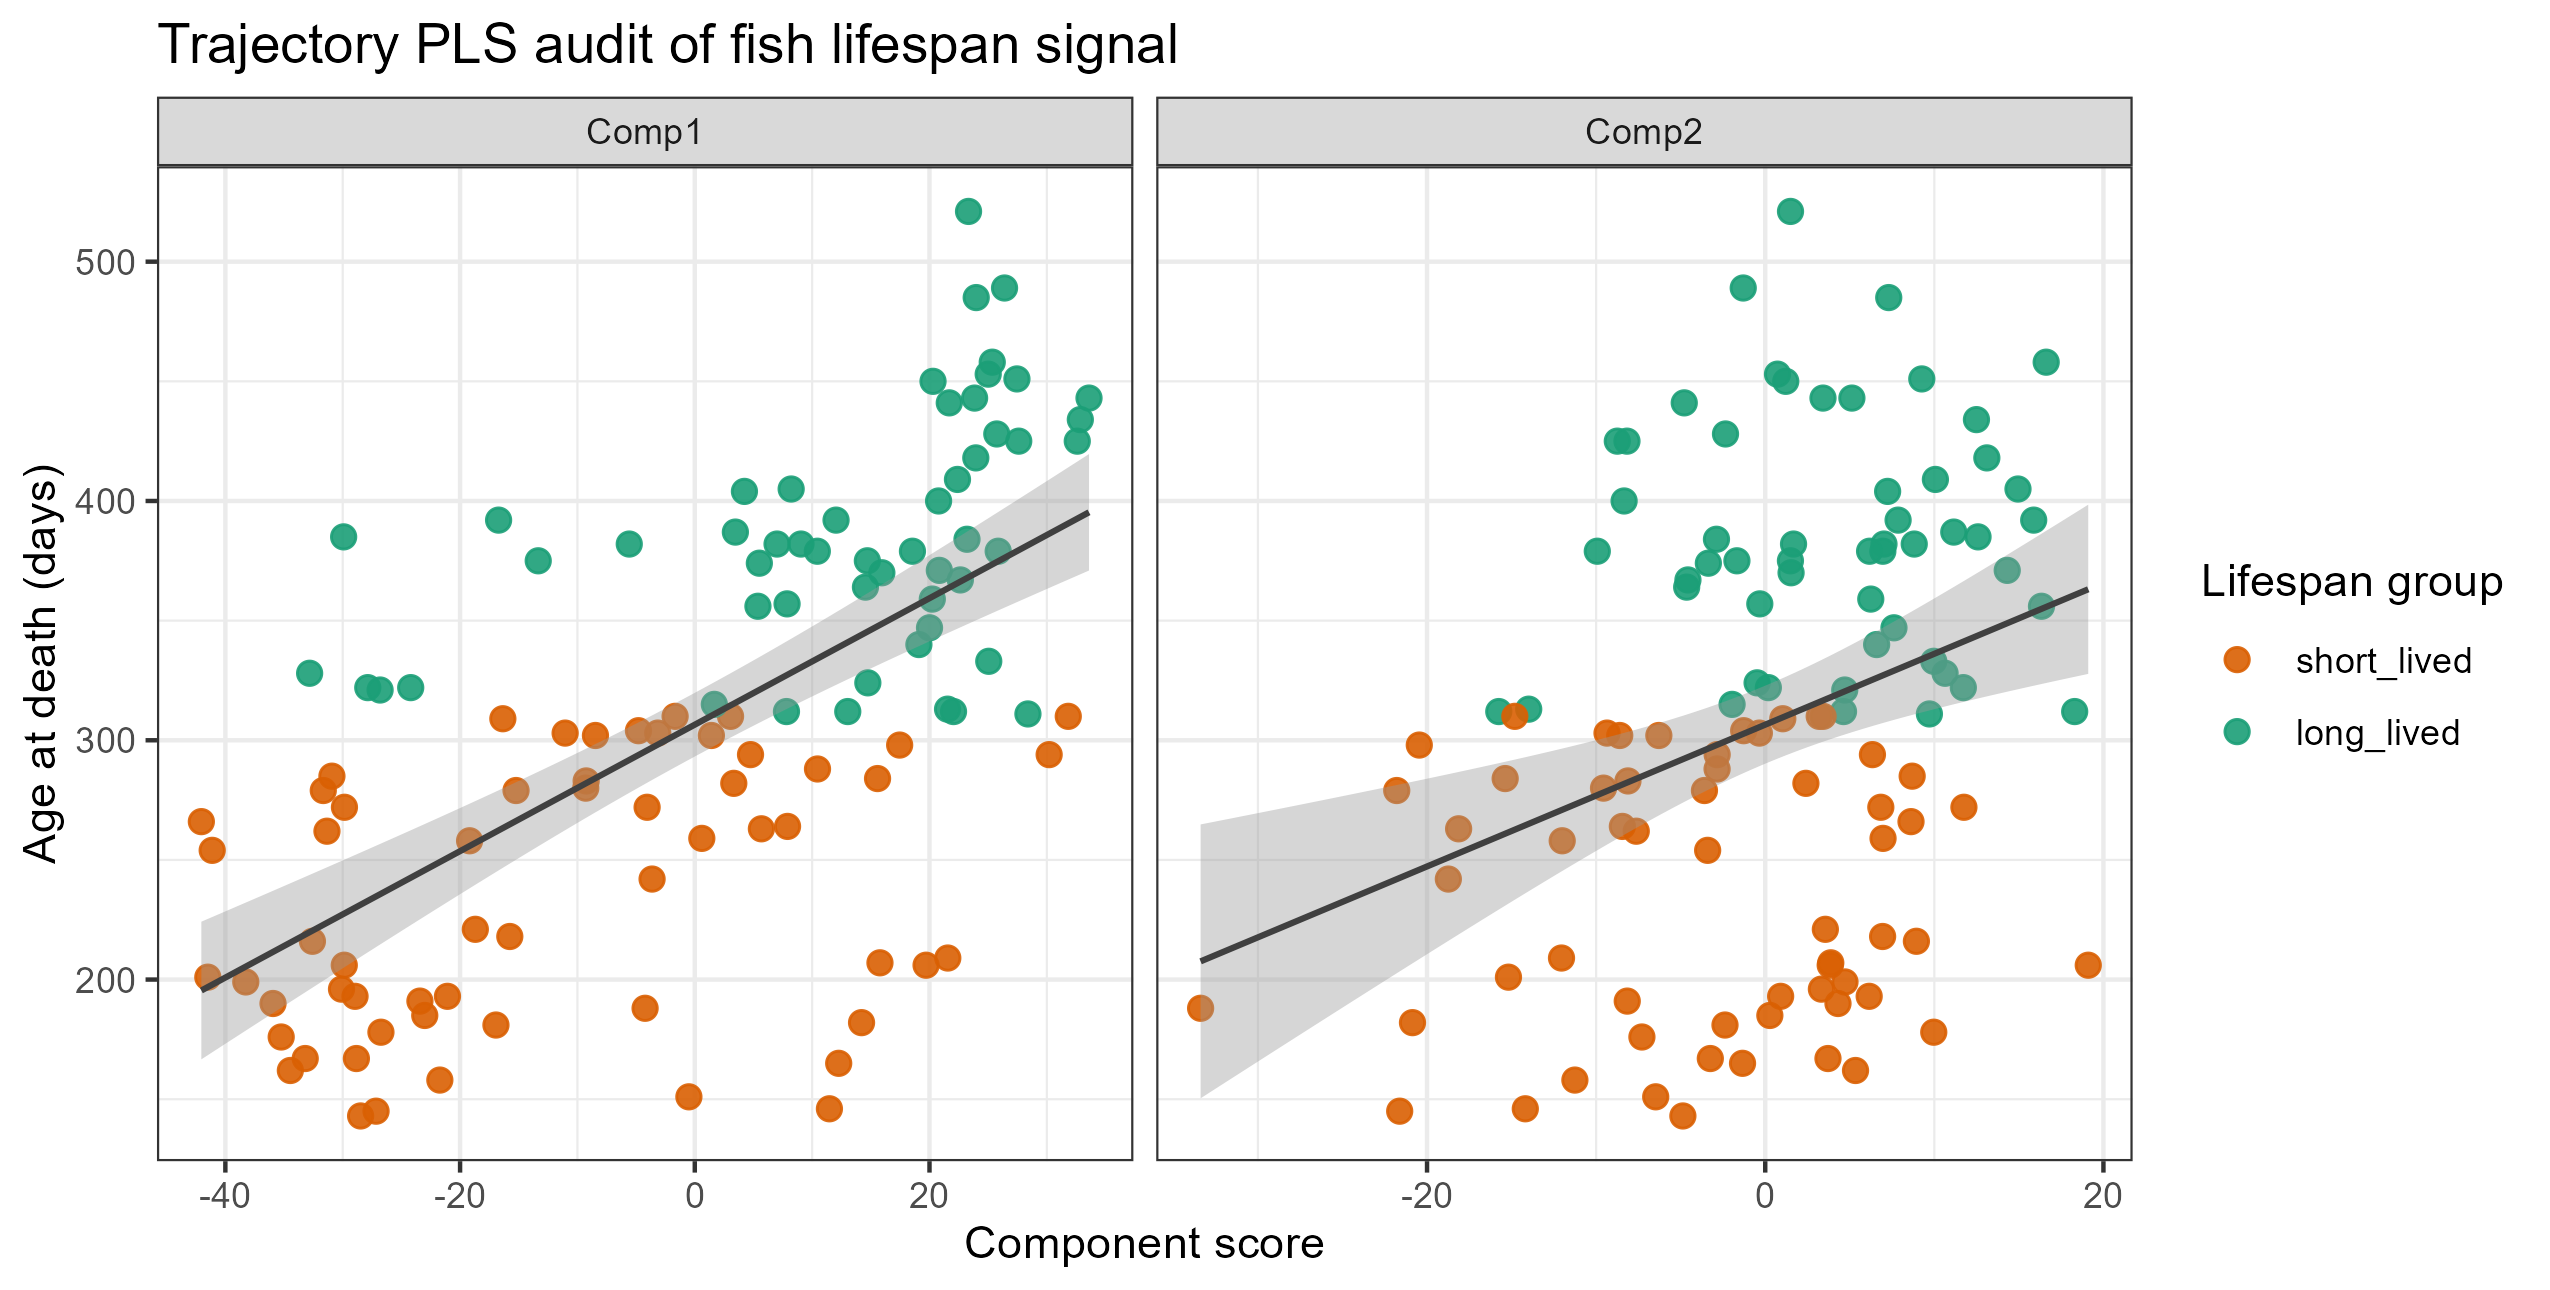
\includegraphics[width=\textwidth]{fish_lifespan_component_correlations.png}
    \caption{Audit component scores against continuous age at death.}
  \end{subfigure}
  \vspace{0.4em}
  \begin{subfigure}{0.43\textwidth}
    \centering
    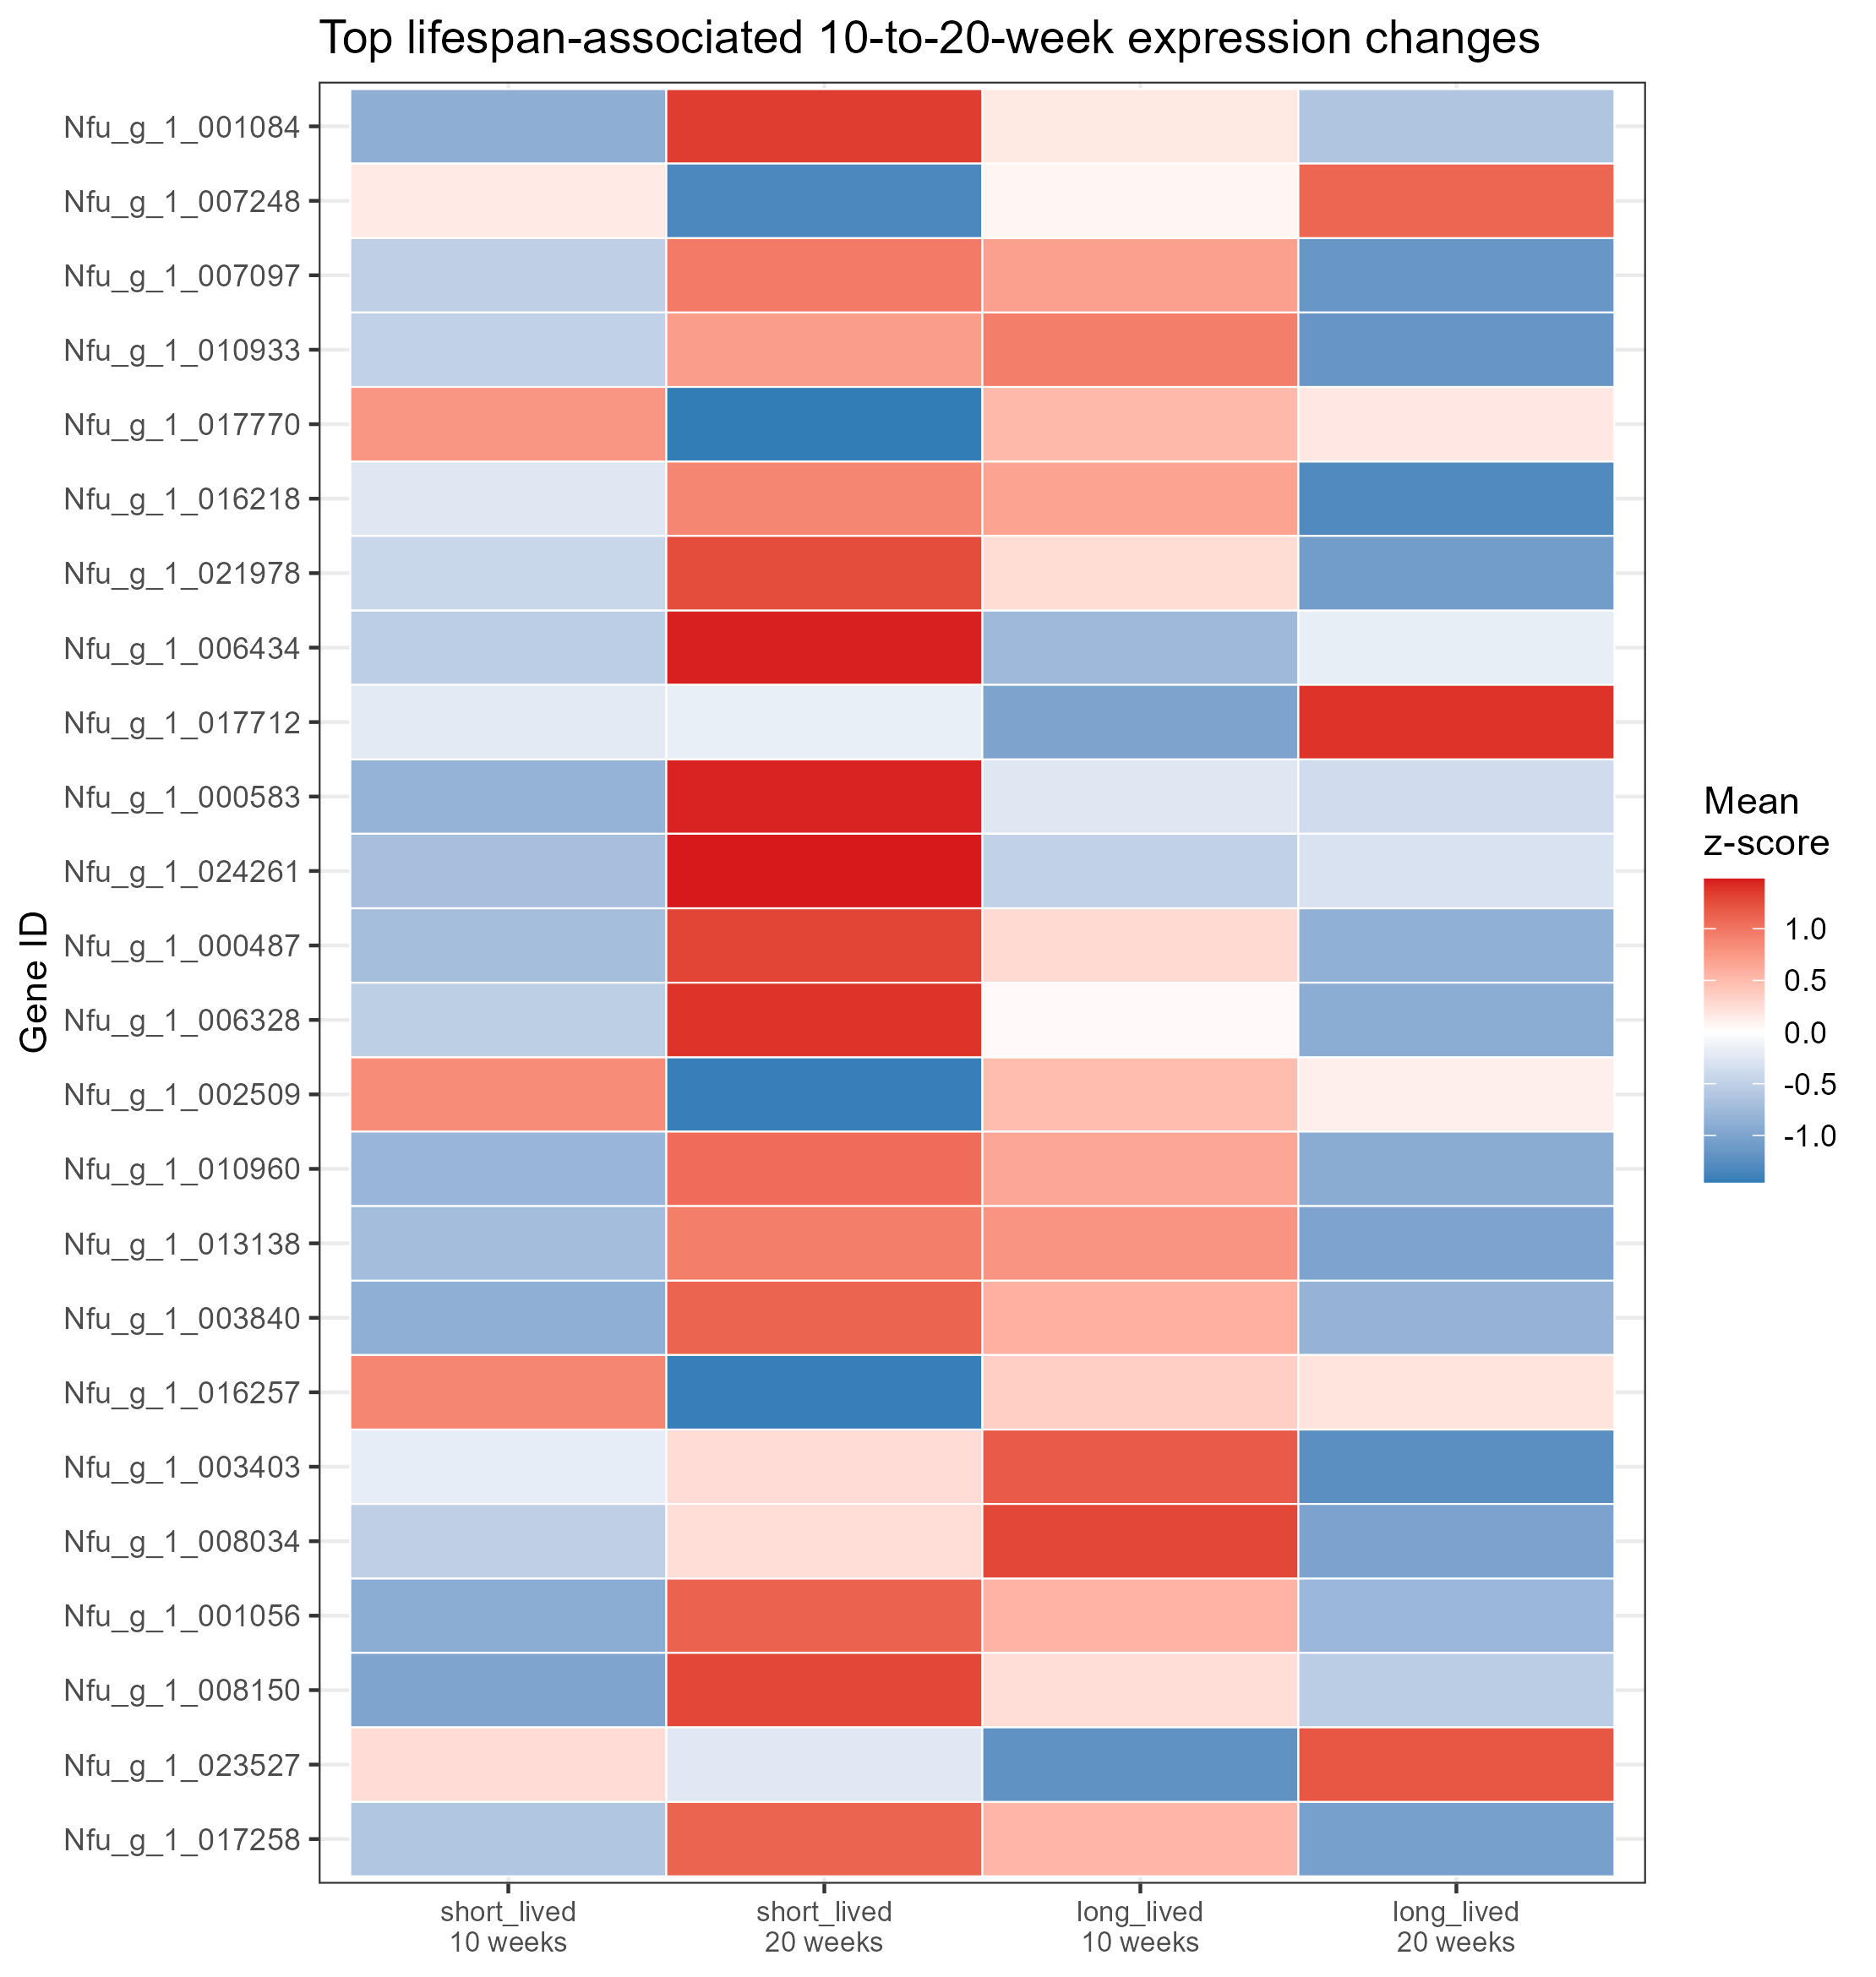
\includegraphics[width=\textwidth]{fish_delta_group_heatmap.png}
    \caption{Mean expression of the strongest 10-to-20-week delta genes.}
  \end{subfigure}
  \hfill
  \begin{subfigure}{0.43\textwidth}
    \centering
    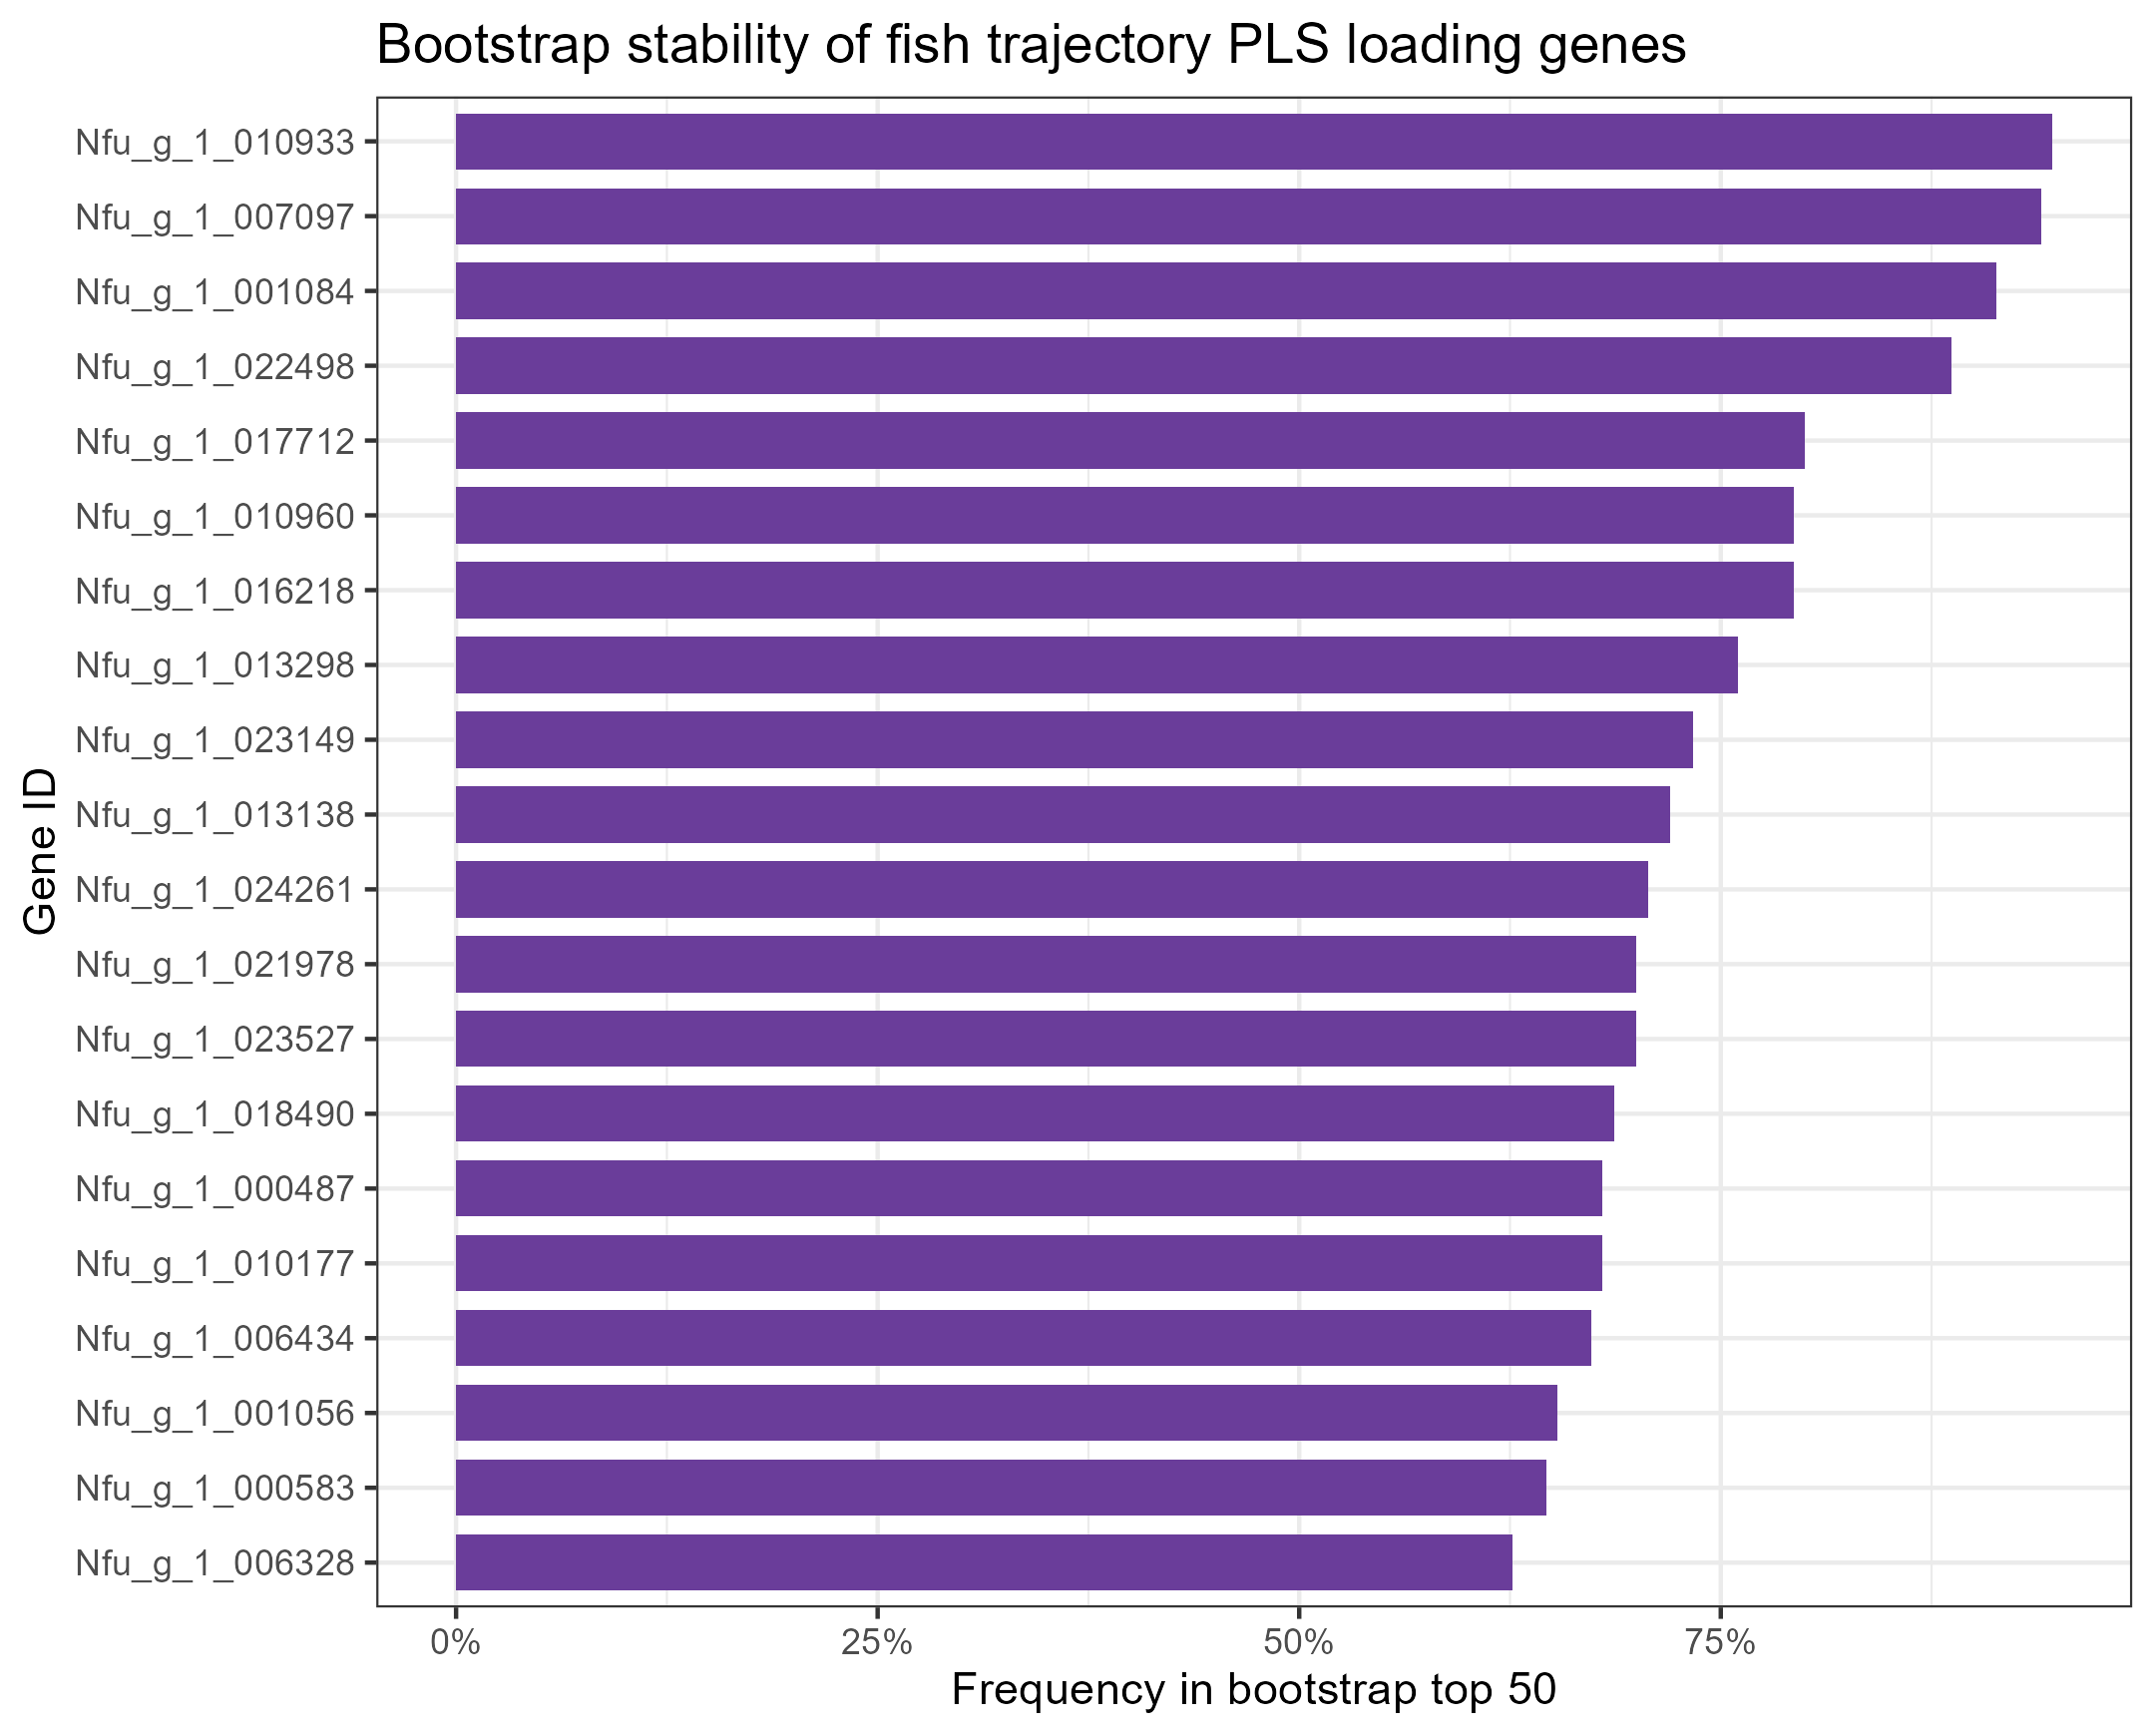
\includegraphics[width=\textwidth]{fish_bootstrap_loading_stability.png}
    \caption{Bootstrap stability of high-loading trajectory genes.}
  \end{subfigure}
  \caption{\textbf{Independent trajectory check of the fish lifespan signal.} The analysis estimated trajectory-level PLS components from local GEO files and evaluated continuous lifespan, group-specific temporal deltas and loading stability.}
  \label{fig:fish_check}
\end{figure}

Figure~\ref{fig:fish_check} gives a more detailed view of the independent analysis. Both components increase with age at death, especially Component 1. The delta heatmap shows that several genes change differently between 10 and 20 weeks in short-lived and long-lived fish. The bootstrap panel adds a stability check: some high-loading genes appeared repeatedly among the top features, which argues against a signal created by one random fit.

This result is consistent with the design of the original dataset. GSE150318 was built to test whether early adult expression profiles contain information about later aging and lifespan \citep{baumgart2016killifish}. My analysis supports that idea statistically. It also suggests that the signal is connected to temporal change, not only to one static expression measurement.

The gene-level interpretation is more delicate. In the original tensorOmics output, the overlap between the top 50 loading genes and the top 50 simple delta genes was 3 out of 50, close to the expected overlap of 2.5 ($p=0.463$). In the independent trajectory analysis, the overlap was 36 out of 50 ($p=5.07\times10^{-43}$), but this is partly expected because the representation explicitly included delta features. These two results are not contradictory. The tensorOmics model captured a broader supervised trajectory pattern, while the independent analysis checked whether group-specific temporal deltas could recover the same lifespan signal.

The main limitation is annotation. Many fish top features remain \texttt{Nfu\_g} identifiers without reliable gene-symbol interpretation in this workflow. Therefore, the result is best written as evidence for lifespan-associated early transcriptomic trajectories, not as evidence for one specific pathway. The mitochondrial complex I mechanism from Baumgart et al. remains the literature background, but I did not reproduce that full mechanism locally.

\FloatBarrier

\subsection{Trajectory PCA separated vaccine subjects by age, but cohort structure had to be controlled}

\begin{figure}[!htbp]
  \centering
  \begin{subfigure}{0.48\textwidth}
    \centering
    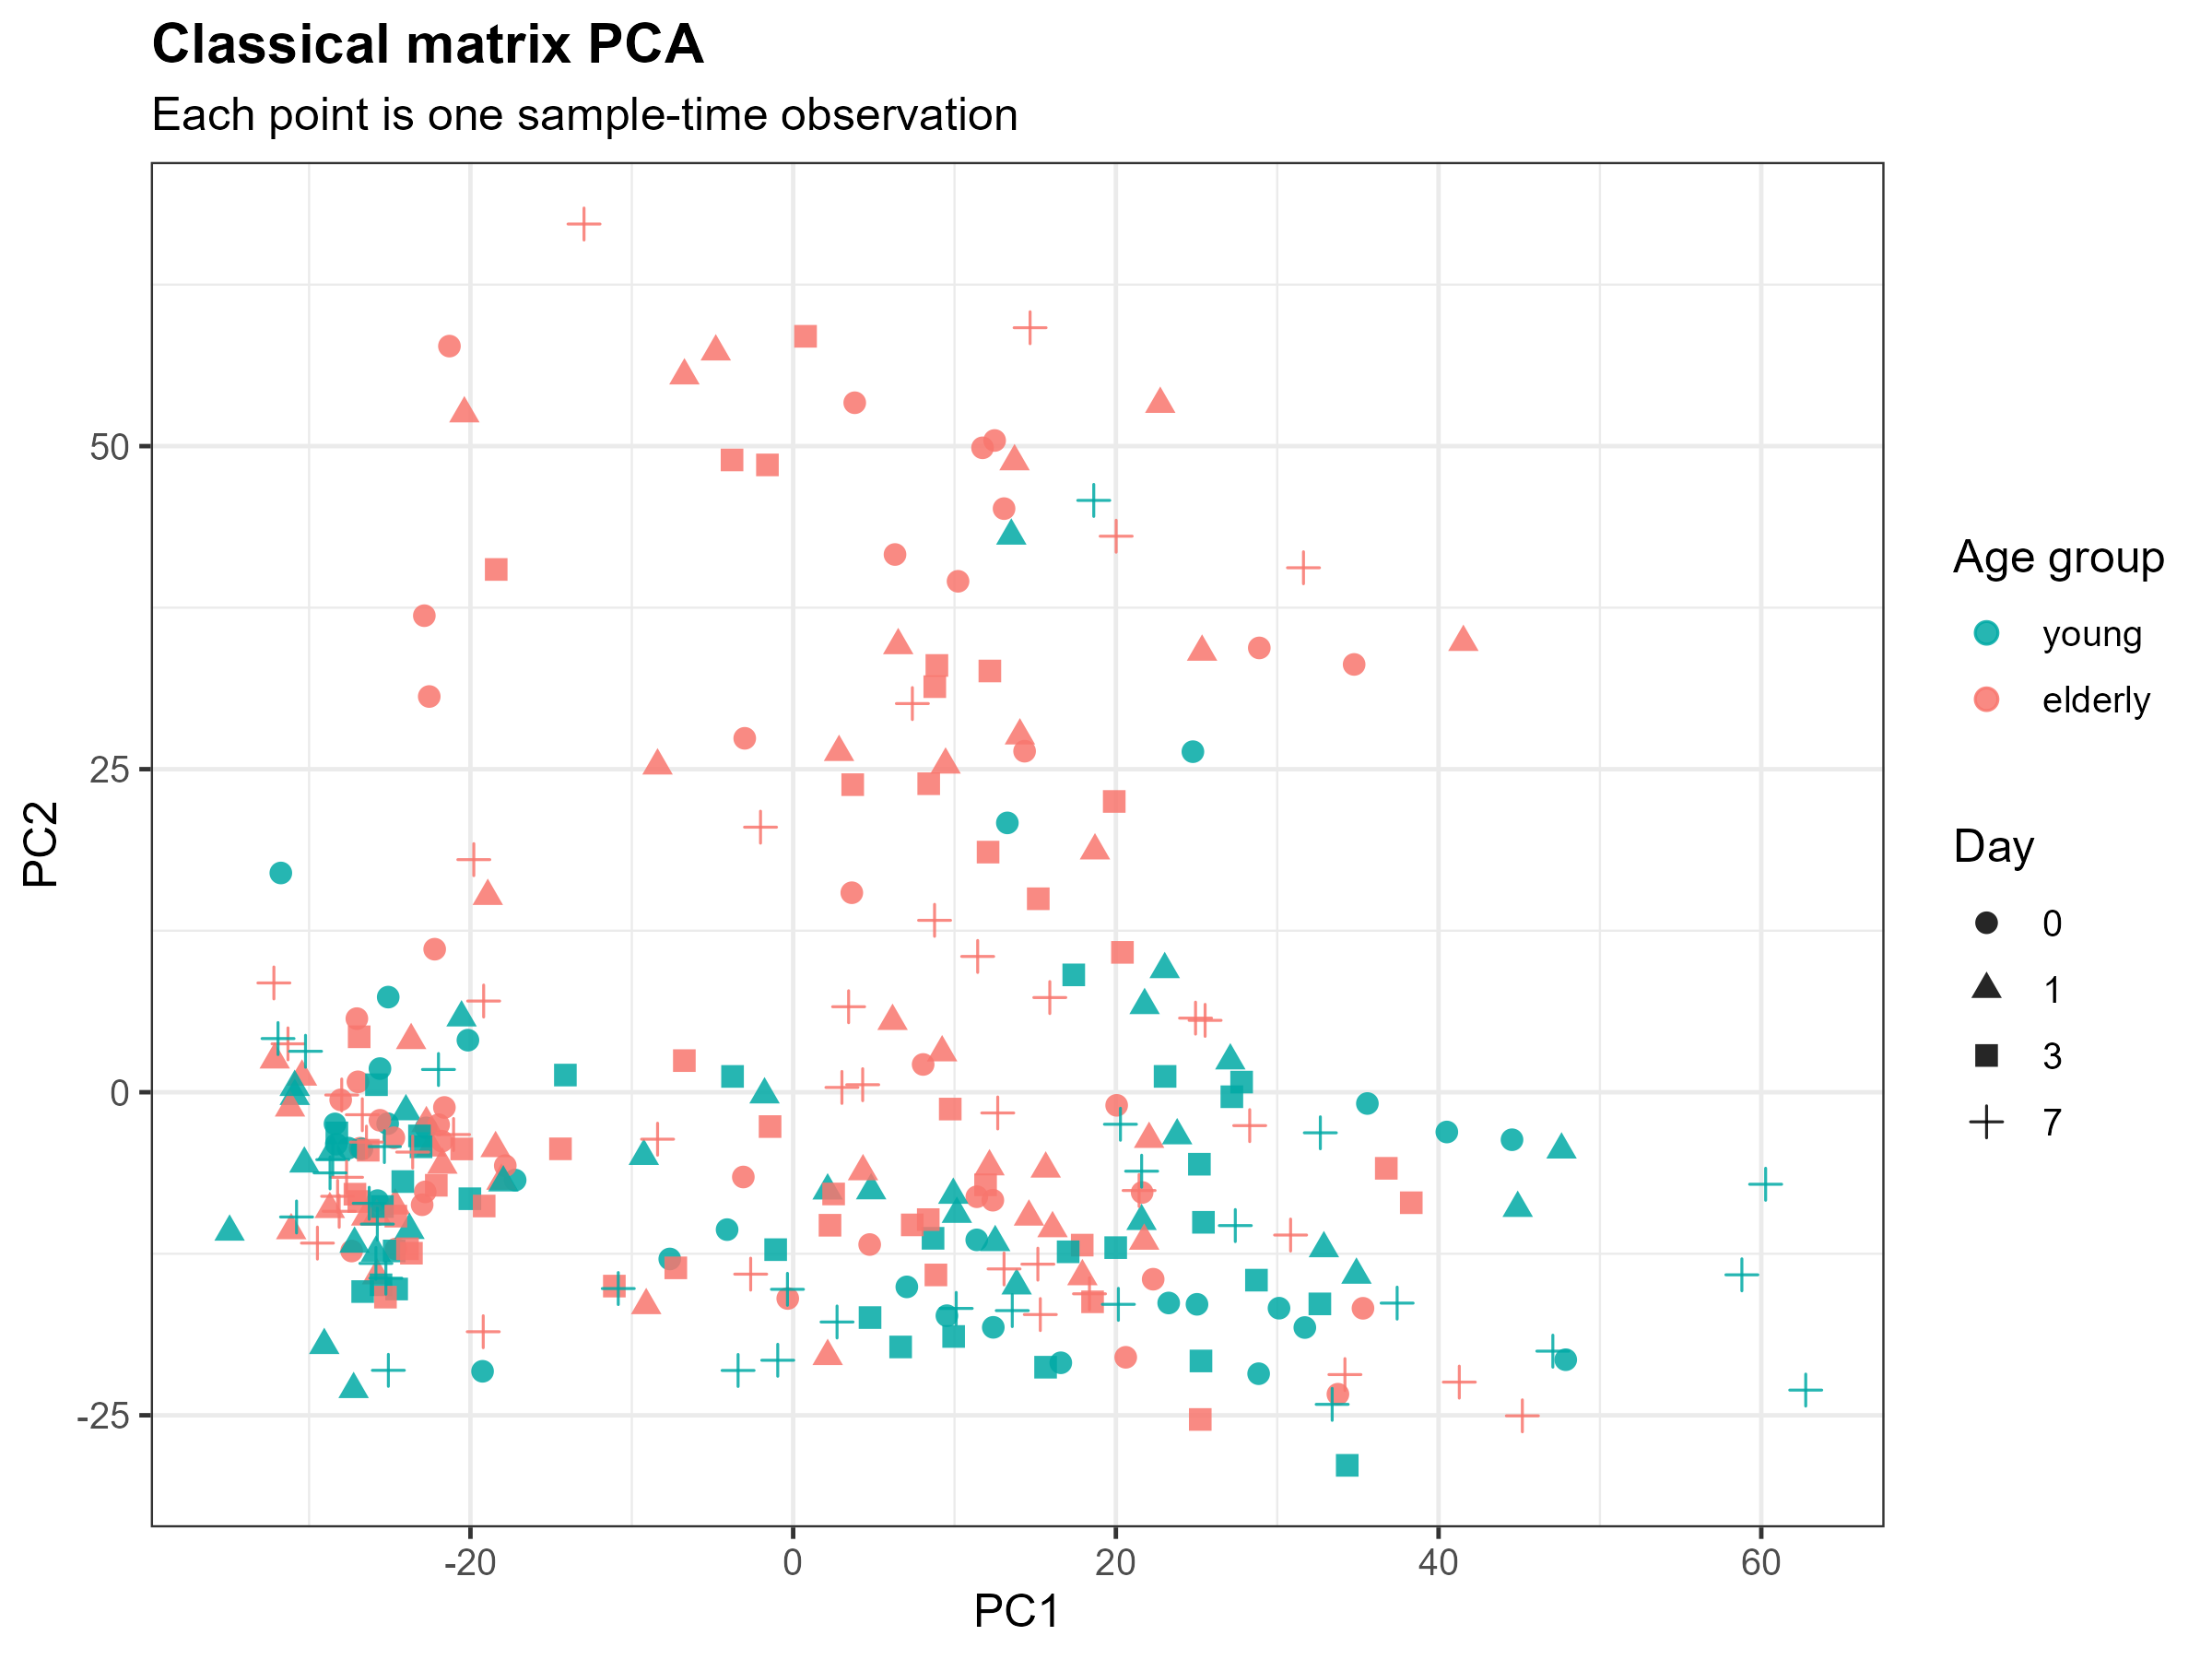
\includegraphics[width=\textwidth]{01_matrix_pca_samples.png}
    \caption{Classical matrix PCA.}
  \end{subfigure}
  \hfill
  \begin{subfigure}{0.48\textwidth}
    \centering
    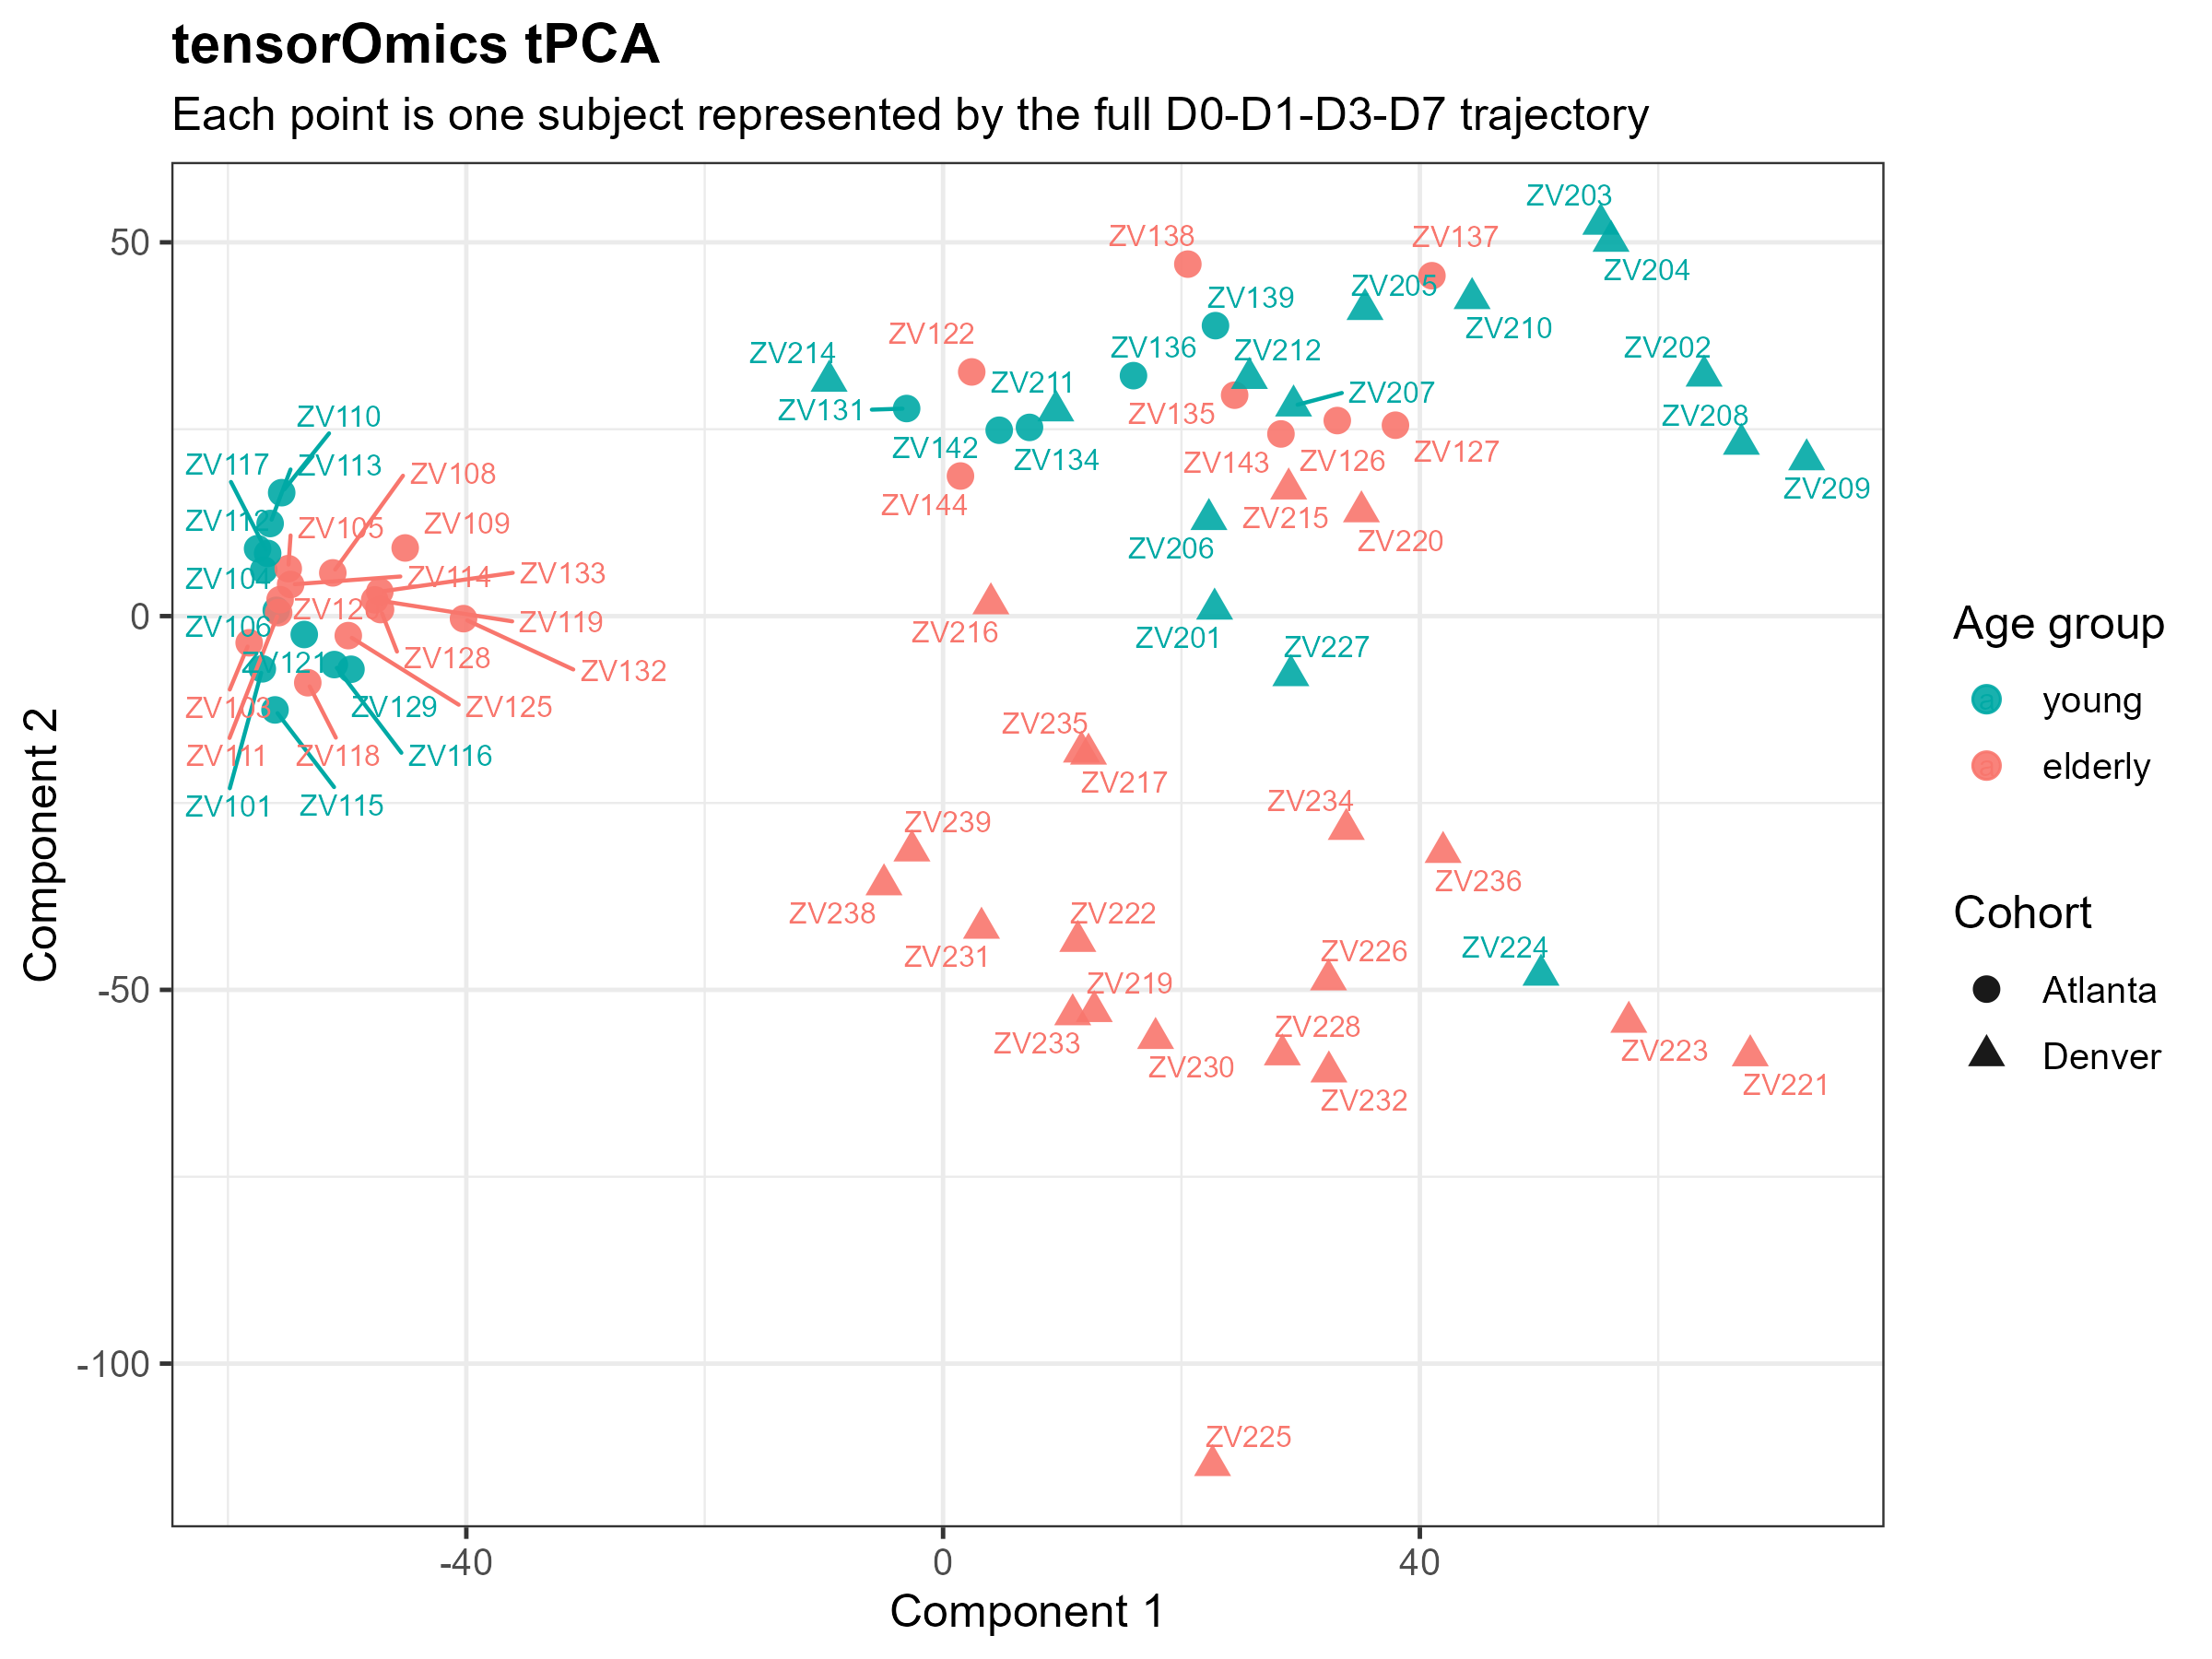
\includegraphics[width=\textwidth]{02_tensor_pca_subjects.png}
    \caption{tensorOmics tPCA.}
  \end{subfigure}
  \caption{\textbf{Matrix and tensor PCA views of GSE79396.} In the matrix PCA, each point is one sample-time observation. In the tPCA plot, each point is one subject represented by the full D0-D1-D3-D7 transcriptomic trajectory. Colours indicate age group and shapes indicate cohort where shown.}
  \label{fig:vaccine_matrix_tensor}
\end{figure}

The vaccine dataset required an extra check for cohort effects. Figure~\ref{fig:vaccine_matrix_tensor}a shows a classical matrix PCA, where each point is one sample-time observation. Young and elderly samples overlap, and the time-point symbols are mixed across the plot. This view shows global variation, but it does not directly show one participant as one longitudinal trajectory.

The tensorOmics tPCA plot in Figure~\ref{fig:vaccine_matrix_tensor}b is easier to read in terms of participants, because each point represents one complete D0-D1-D3-D7 trajectory. Age-group separation is visible, especially along Component 2. At the same time, the plot also shows cohort structure: many right-side points are Denver subjects, while Atlanta subjects are more compact on the left. This prevented a wrong interpretation of PC1 as a simple age axis. The tensor plot made the subject-level structure visible, but it also showed that age and cohort effects had to be separated.

The original tensorOmics tPCA score test found an age-group association using Components 1 and 2 (Pillai's trace $=0.186$, $p=8.09\times10^{-4}$; permutation $p=0.002$). The subject-averaged matrix PCA also found an age association ($p=9.72\times10^{-4}$; permutation $p=0.004$), so the matrix baseline was not uninformative. Component-level testing clarified the tensor result: Component 1 was not associated with age group ($p=0.932$), whereas Component 2 was ($p=1.53\times10^{-4}$).

\begin{figure}[!htbp]
  \centering
  \begin{subfigure}{0.54\textwidth}
    \centering
    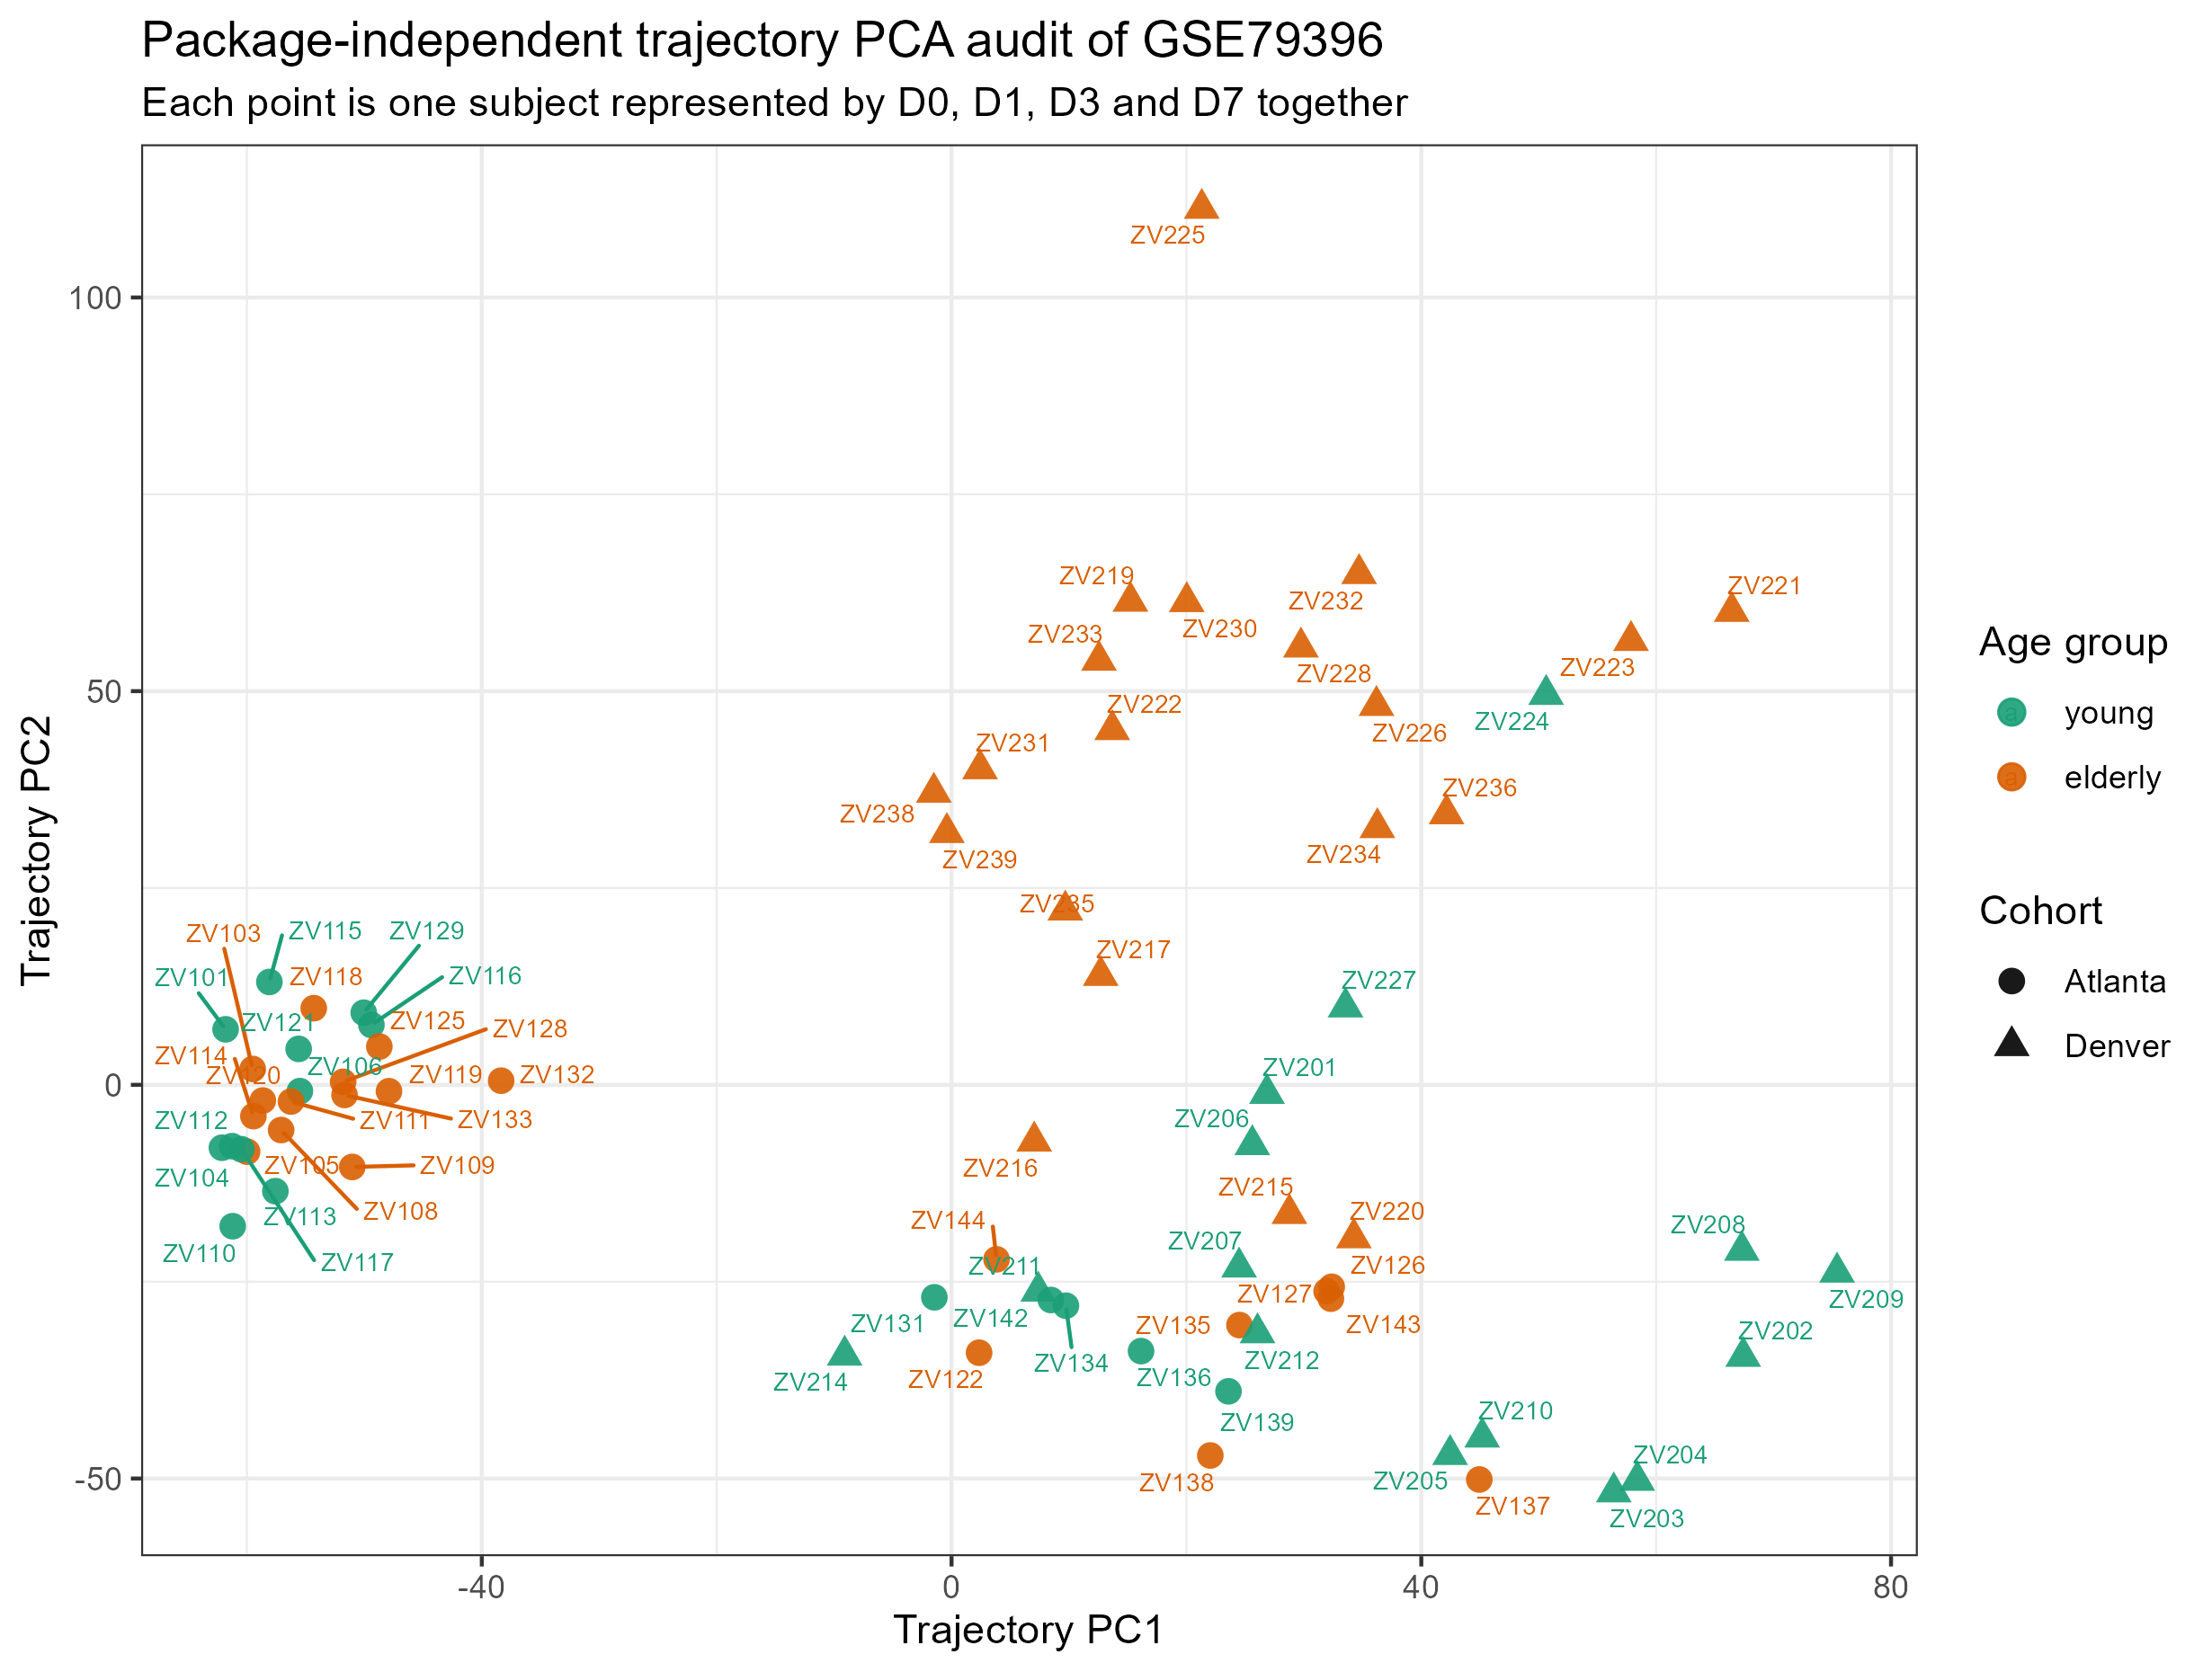
\includegraphics[width=\textwidth]{vaccine_trajectory_pca_scores.png}
    \caption{Package-independent trajectory PCA.}
  \end{subfigure}
  \hfill
  \begin{subfigure}{0.35\textwidth}
    \centering
    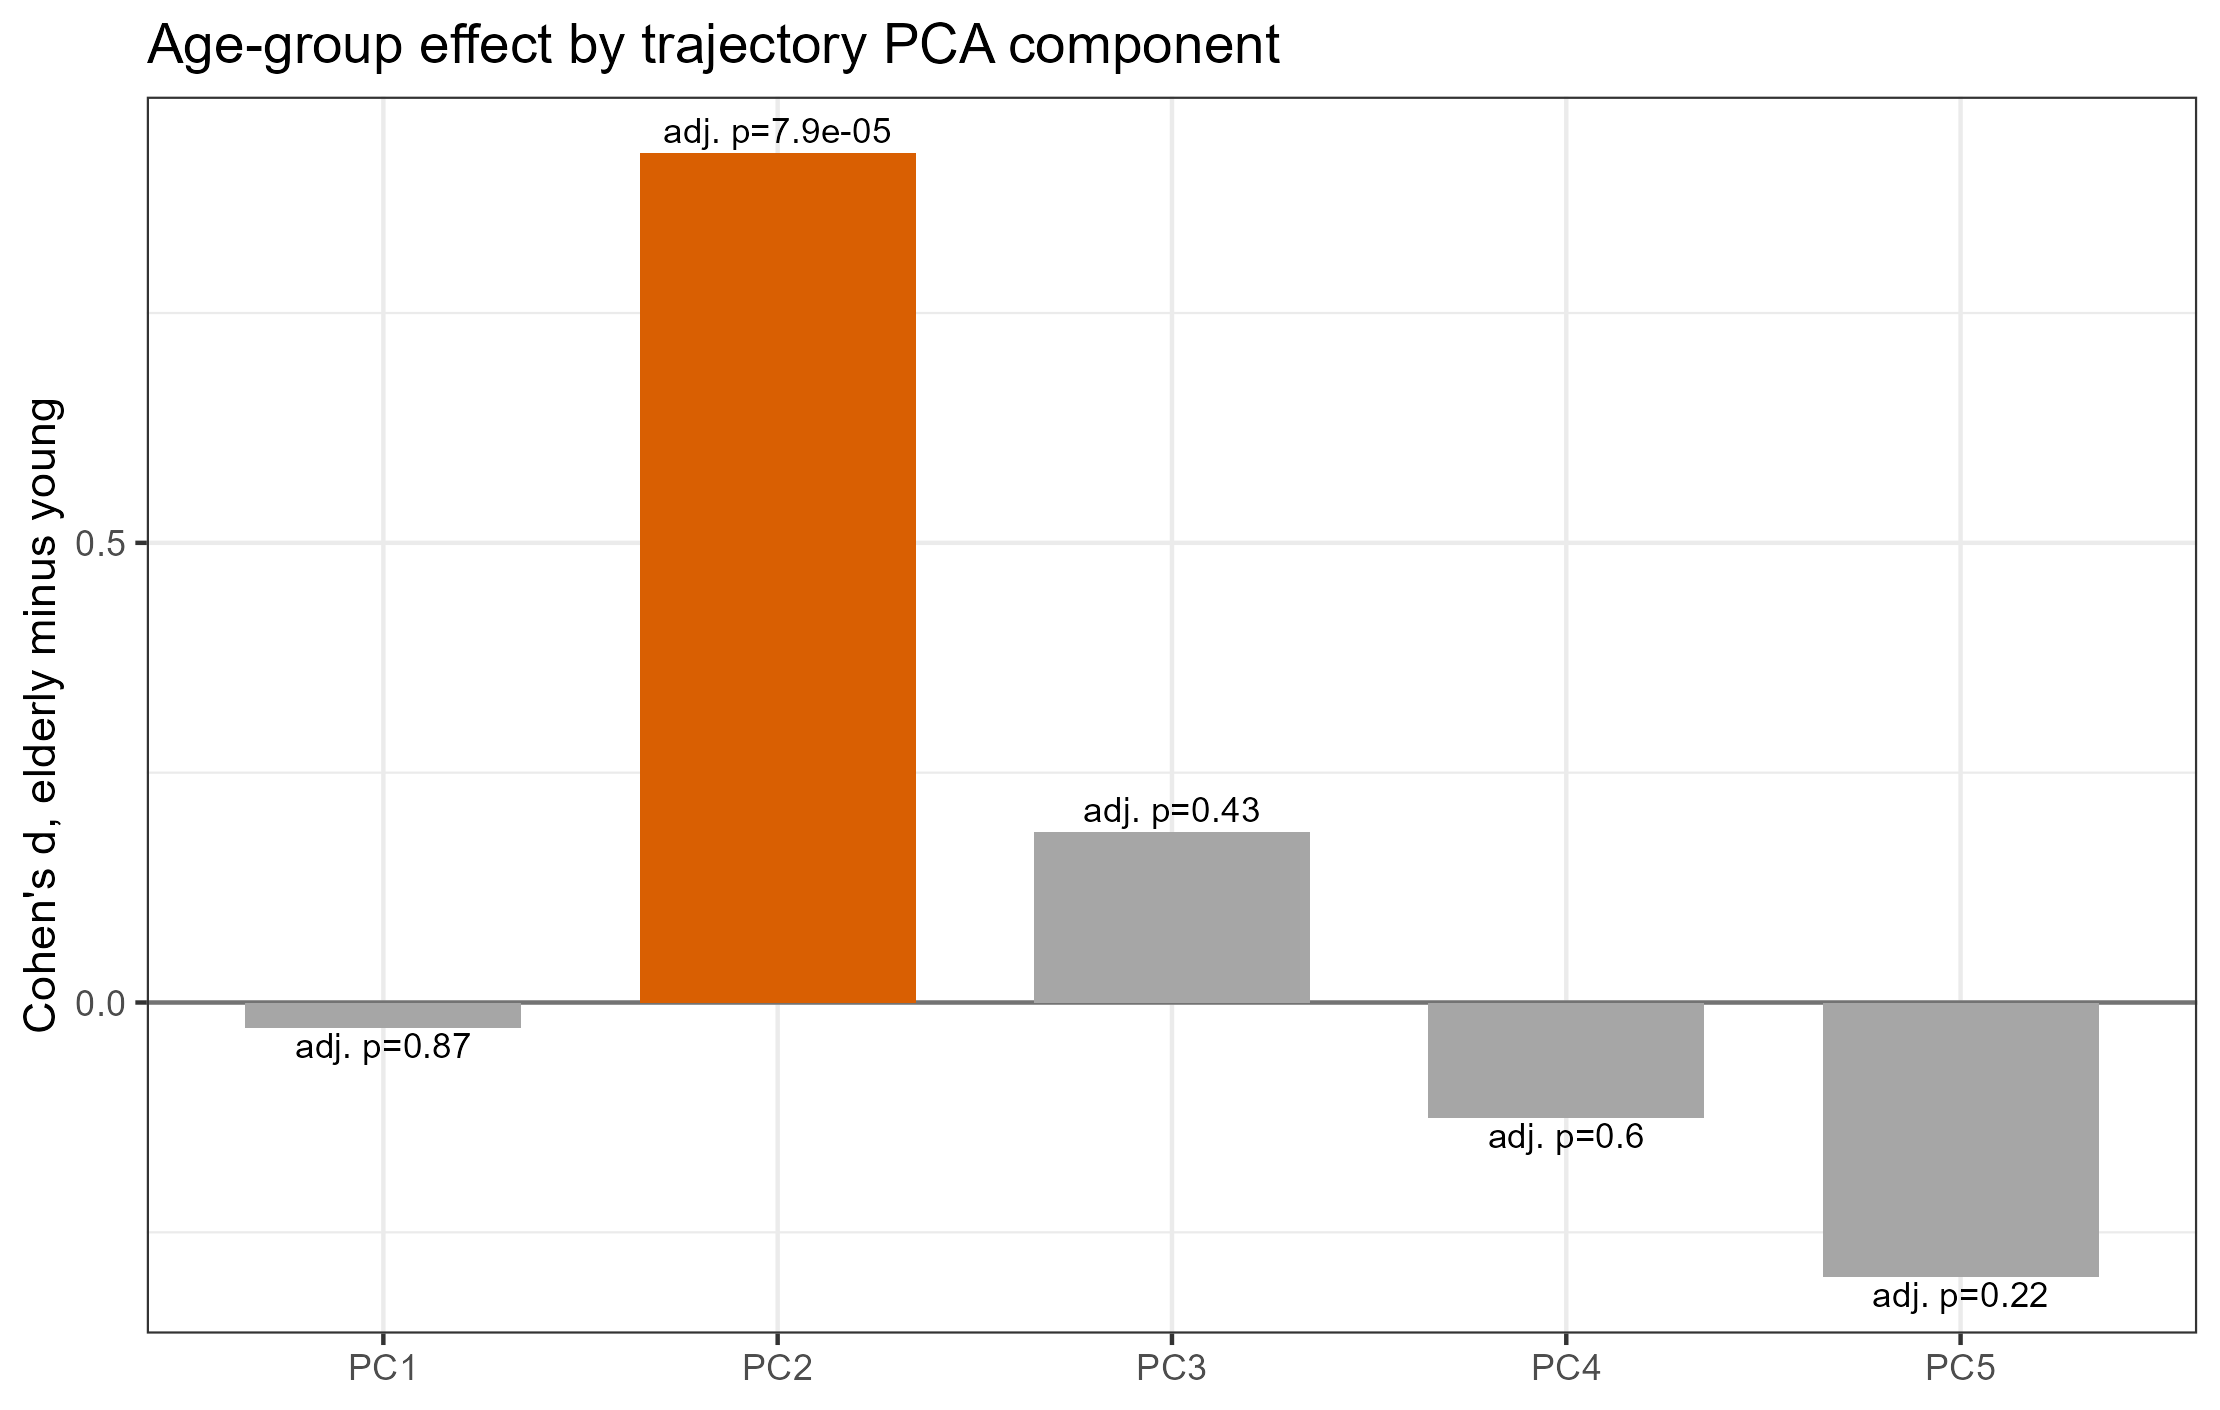
\includegraphics[width=\textwidth]{vaccine_age_effects_by_component.png}
    \caption{Age effect by trajectory component.}
  \end{subfigure}
  \caption{\textbf{Independent check of the age-associated vaccine trajectory component.} The analysis used the same subject-level D0-D1-D3-D7 structure but did not call tensorOmics.}
  \label{fig:vaccine_check}
\end{figure}

The independent trajectory analysis reproduced the age-group signal (PC1-PC2 MANOVA $p=0.00119$; permutation $p=0.001$). It also made the confounding structure explicit. After adjustment for cohort and sex, PC2 was the only component with an age effect (elderly minus young Cohen's $d=0.924$, adjusted $p=7.91\times10^{-5}$). PC1 had no adjusted age effect ($p=0.871$), but cohort was strongly associated with PC1 in the same model ($p=1.20\times10^{-11}$). The defensible interpretation is specific: PC1 mainly reflects cohort or other structured variation, while PC2 carries the age-associated transcriptomic trajectory.

\subsection{The vaccine PC2 axis was enriched for inflammatory, oxidative and lipid or sterol signals}

\begin{figure}[!htbp]
  \centering
  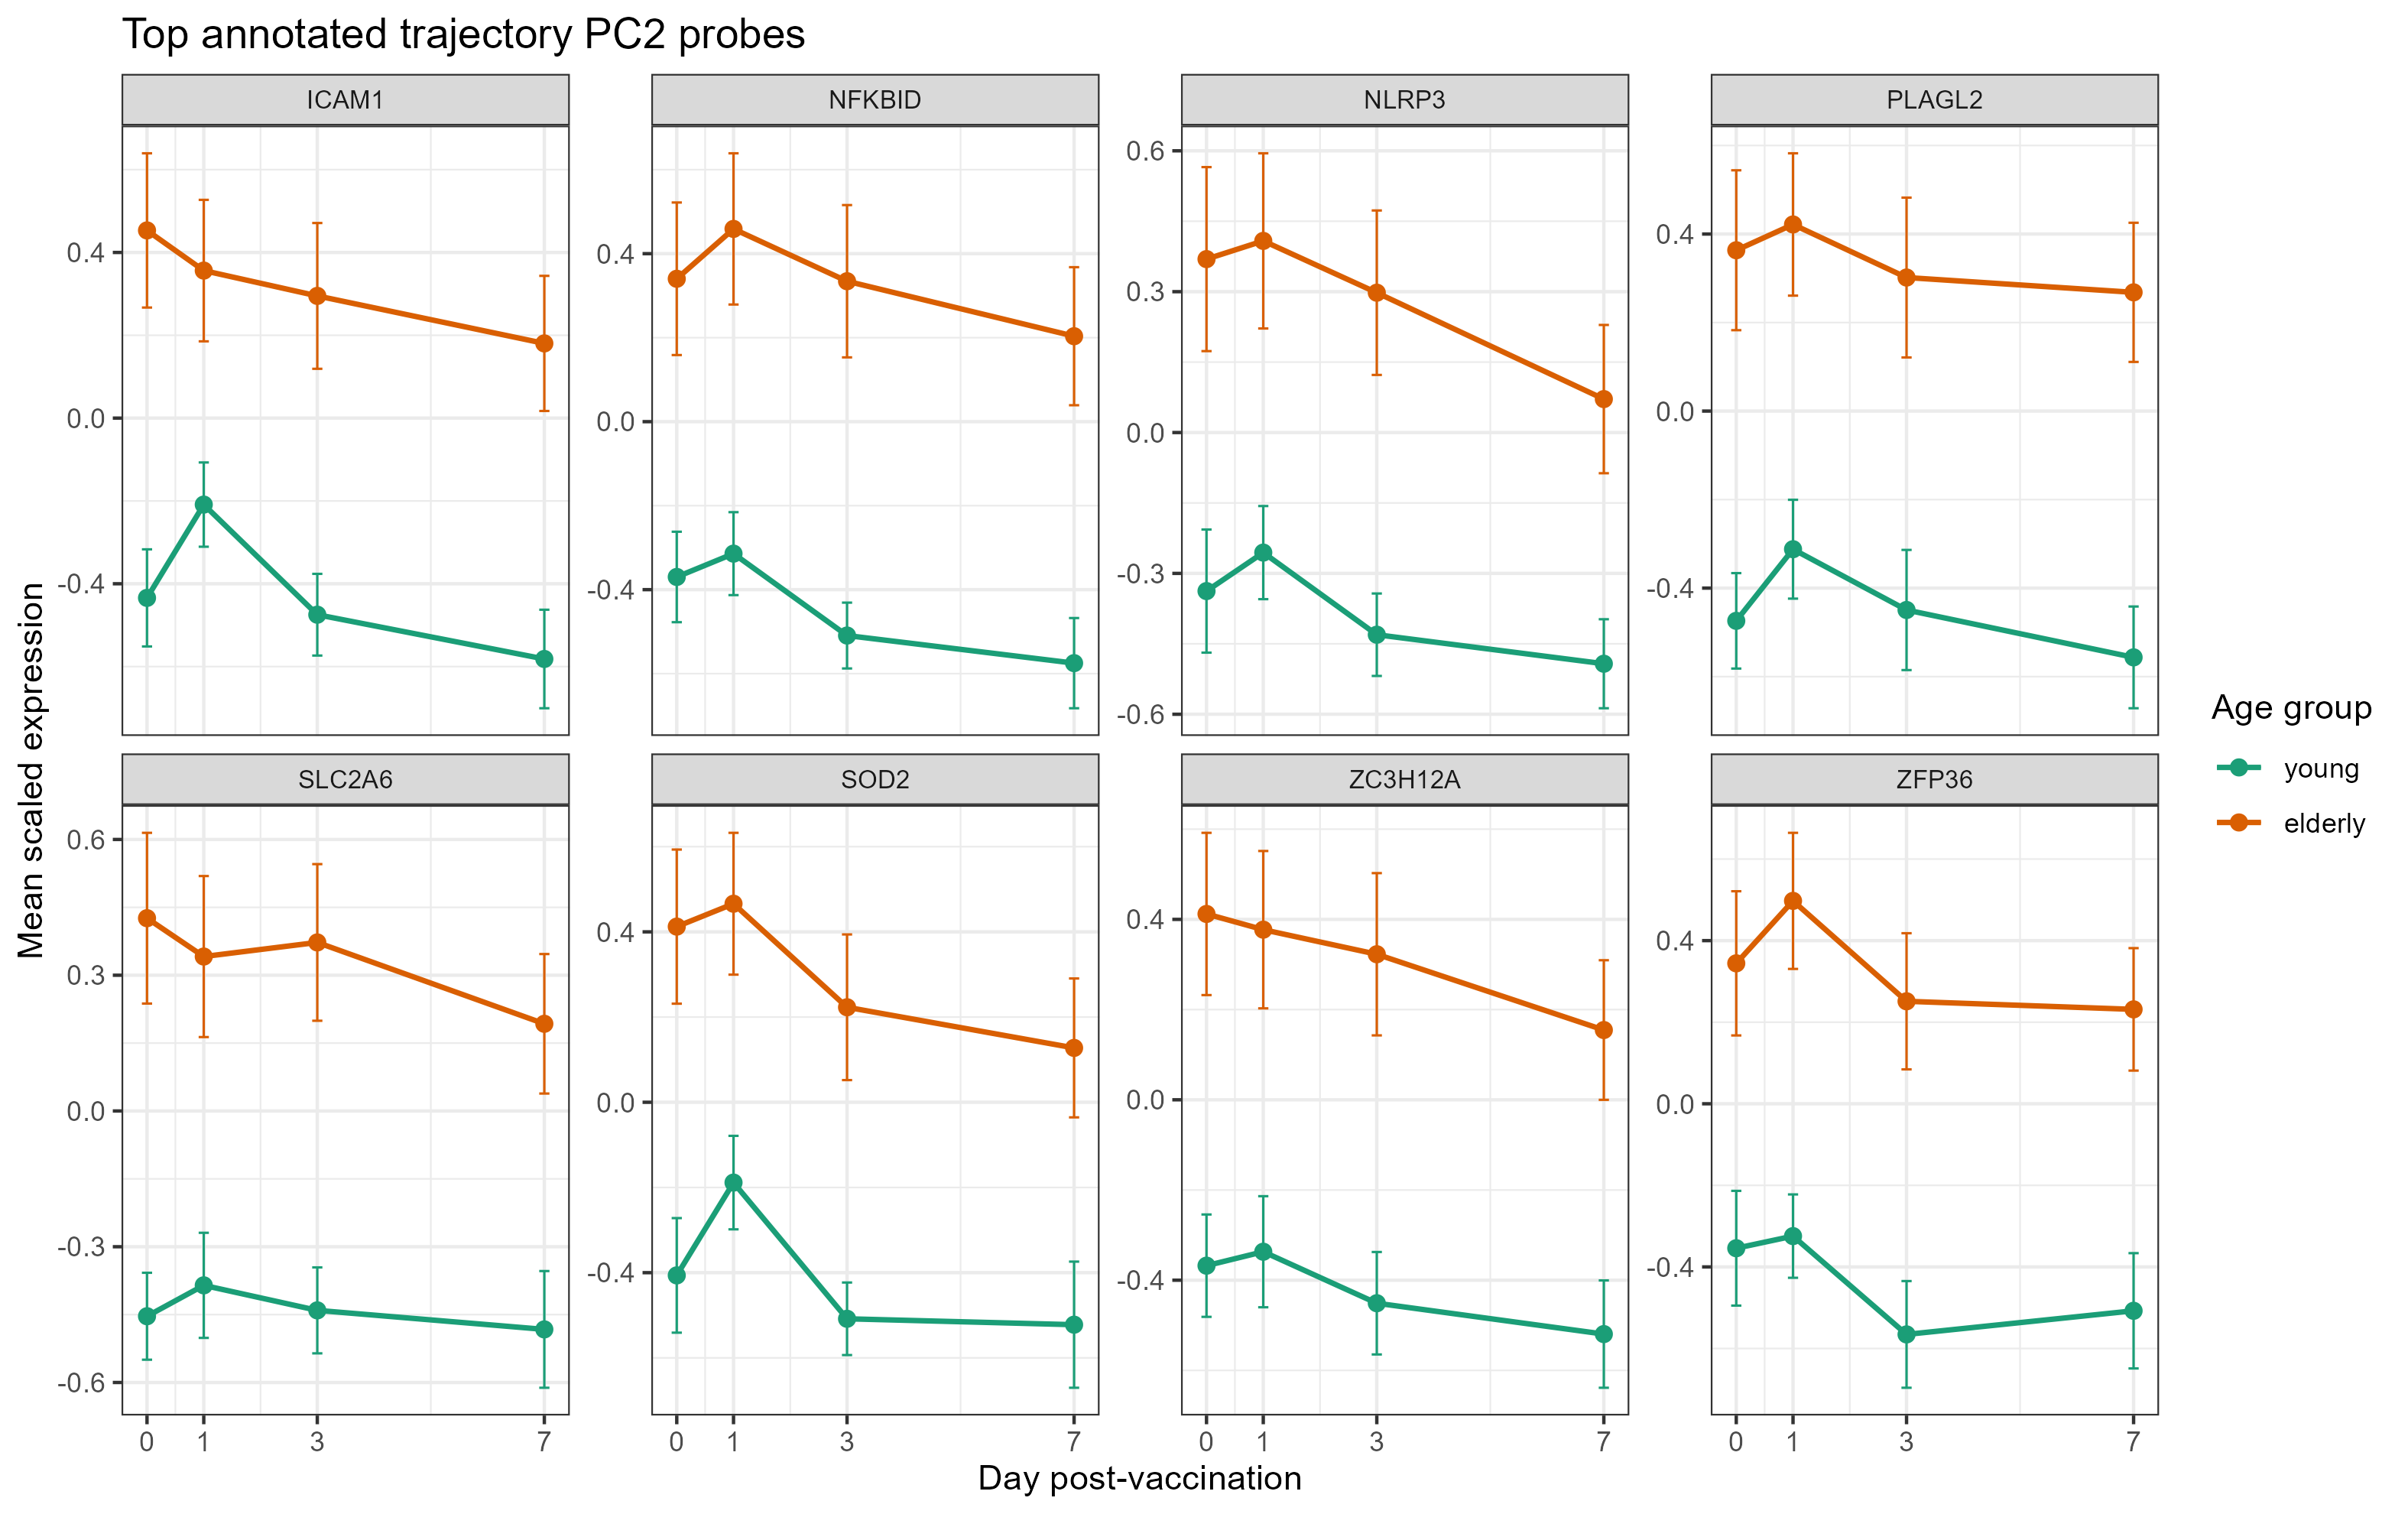
\includegraphics[width=0.88\textwidth]{vaccine_pc2_top_gene_trajectories_annotated.png}
  \caption{\textbf{Top annotated trajectory PC2 probes in GSE79396.} Each panel shows mean scaled expression across days 0, 1, 3 and 7 for one annotated high-loading PC2 gene. Points and error bars summarize age-group means and standard errors.}
  \label{fig:vaccine_gene_trajectories}
\end{figure}

The vaccine probes allowed a more direct biological reading than the fish identifiers. Figure~\ref{fig:vaccine_gene_trajectories} shows eight annotated high-loading PC2 genes. Elderly subjects have higher mean scaled expression than young subjects for \textit{ICAM1}, \textit{NFKBID}, \textit{NLRP3}, \textit{PLAGL2}, \textit{SLC2A6}, \textit{SOD2}, \textit{ZC3H12A} and \textit{ZFP36}. The age difference is already present at day 0 and remains visible across days 1, 3 and 7. The dominant pattern is a persistent age-group offset, rather than a clean short post-vaccination pulse.

The gene identities give PC2 a plausible biological reading. \textit{ICAM1} is linked to leukocyte adhesion and inflammatory signalling. \textit{SOD2} is related to mitochondrial oxidative-stress handling. \textit{ZFP36} and \textit{ZC3H12A} regulate inflammatory mRNA stability, and \textit{NLRP3} and \textit{IL1B} belong to innate inflammatory pathways. These genes do not prove a mechanism by themselves, but they make the age-associated PC2 axis compatible with an inflammatory and stress-related transcriptomic state in older adults.

\begin{table}[!htbp]
  \centering
  \caption{\textbf{Keyword enrichment among the top 100 trajectory PC2 probes.}}
  \label{tab:vaccine_keyword}
  \footnotesize
  \begin{tabular}{lrrrr}
    \toprule
    Category & Top hits & Odds ratio & $p$ value & FDR \\
    \midrule
    Inflammatory or innate immune terms & 41/100 & 2.29 & $1.62\times10^{-4}$ & $6.49\times10^{-4}$ \\
    Oxidative-stress terms & 8/100 & 2.71 & 0.0166 & 0.0221 \\
    Lipid or sterol terms & 13/100 & 2.55 & 0.00673 & 0.0135 \\
    Antigen-presentation terms & 3/100 & 1.44 & 0.473 & 0.473 \\
    \bottomrule
  \end{tabular}
\end{table}

The keyword enrichment points in the same direction. Among the top 100 PC2 probes, inflammatory or innate immune terms were enriched at 41 out of 100 probes (odds ratio 2.29, FDR $=6.49\times10^{-4}$). Oxidative-stress terms and lipid or sterol terms were also enriched after correction. Antigen-presentation terms were not enriched (FDR $=0.473$), so the PC2 signal should not be generalized to all immune pathways.

This pattern is consistent with Li et al., who reported age-related inflammatory and innate immune modules and linked sterol-related biology to antibody and Tfh responses \citep{li2017vaccine}. My local analysis extends that interpretation only modestly: it shows that an age-associated early transcriptomic trajectory can be recovered from the GEO expression matrix alone. It does not reproduce the full multi-omic network or establish that PC2 drives vaccine responsiveness.

\subsection{Response-level models did not pass validation}

\begin{figure}[!htbp]
  \centering
  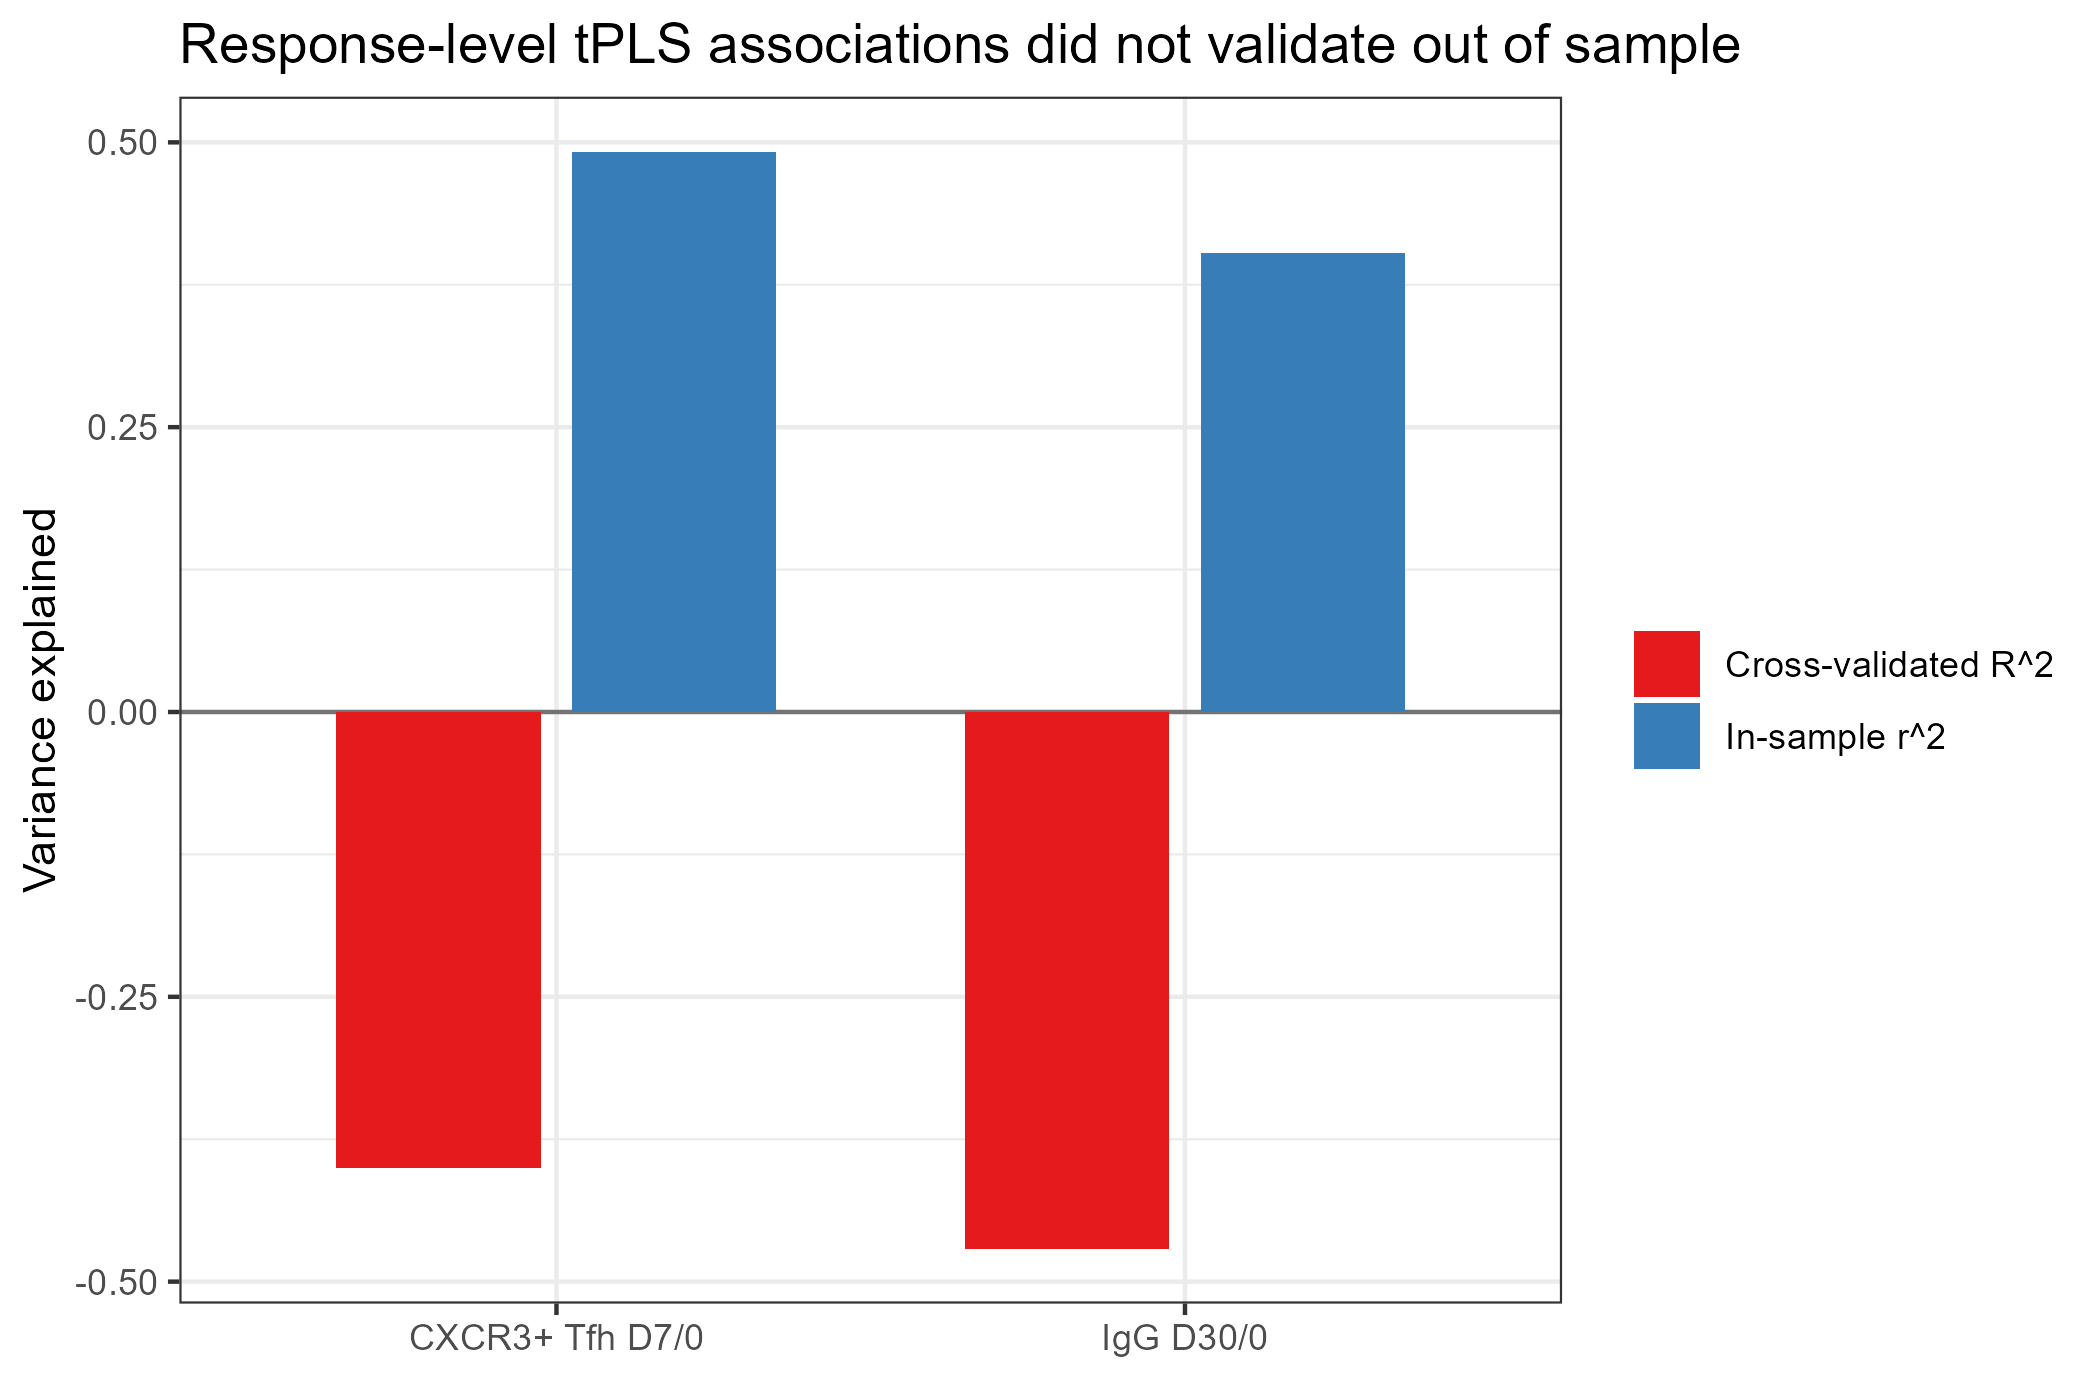
\includegraphics[width=0.60\textwidth]{vaccine_response_validation_summary.png}
  \caption{\textbf{Response-level tPLS associations did not validate out of sample.} Blue bars show in-sample variance explained by response-level tPLS Component 1. Red bars show cross-validated $R^2$.}
  \label{fig:vaccine_response}
\end{figure}

The response-level models show why validation was needed. In-sample correlations were high: IgG D30/0 had $r=0.635$ ($p=3.67\times10^{-9}$), and CXCR3+ Tfh D7/0 had $r=0.701$ ($p=3.82\times10^{-6}$). On their own, these numbers would suggest a response-prediction signal.

The validation checks changed that reading. The permutation $p$ values were 0.23 for IgG and 0.40 for CXCR3+ Tfh, and the cross-validated $R^2$ values were negative. The independent PC2 score also did not correlate with IgG D30/0 ($r=-0.058$, $p=0.635$) or CXCR3+ Tfh D7/0 ($r=0.120$, $p=0.500$). I therefore did not treat response-level tPLS as a validated predictor. This result fixes the scope of the vaccine analysis: the dataset supports an age-associated transcriptomic trajectory, but not a robust prediction of antibody or Tfh outcome in this workflow.

\FloatBarrier

\section{Discussion}

\subsection{What trajectory-aware analysis added}

The tensor analyses did not simply outperform the matrix baselines. Matrix methods also found structure, especially in the vaccine dataset. The difference was the unit represented in the score plot. In the fish analysis, each point represented a two-time-point expression trajectory and could be related directly to age at death. In the vaccine analysis, each point represented one participant's early post-vaccination trajectory, which made cohort structure visible before biological interpretation.

This matters because longitudinal omics studies often have many more features than subjects. If each sample-time observation is treated as independent, the plot may look richer while partly hiding repeated-measure structure. The tensor view forces the interpretation back to the subject level, but it does not remove confounding. Cohort, sex, baseline state and missing visits can still shape the components.

\subsection{Fish aging interpretation}

The fish results support the working hypothesis that early adult fin transcriptomic trajectories contain information about later lifespan. Both the original tPLS-DA and the independent trajectory analysis explained about half of the variance in age at death using two components. The continuous lifespan association also reduces the chance that the result is only a median-split artifact.

The biological interpretation remains narrow. The original Baumgart study connected longitudinal killifish transcriptomics to aging mechanisms, including mitochondrial complex I \citep{baumgart2016killifish}. My workflow did not recover enough gene annotation to make a comparable mechanism claim. I can claim that the trajectory score captures reproducible lifespan-associated expression patterns among the selected genes. A pathway-level claim would require mapping the \texttt{Nfu\_g} identifiers to current genome annotation, testing enrichment, and checking whether the same genes remain stable under alternative normalization or feature-selection thresholds.

\subsection{Vaccine aging interpretation}

The vaccine PC2 axis can be interpreted at gene level because the top probes are annotated. Elderly subjects showed higher expression of genes linked to inflammatory signalling, oxidative stress and lipid or sterol biology across the early vaccination window. This pattern fits the original Li et al. report, where age-related inflammatory networks and sterol-linked modules were part of the systems-vaccinology model \citep{li2017vaccine}. The local keyword enrichment adds a compact transcriptomic check: the top PC2 probes were not a random list of immune-adjacent genes, and inflammatory terms were enriched after FDR correction.

At the same time, the result is better described as an age-associated transcriptomic state than as a vaccine-response predictor. The age separation was visible at day 0, and the top gene trajectories often showed persistent group offsets. The response models did not validate out of sample, so the local data do not support using this axis to predict IgG or Tfh outcomes.

\subsection{Limitations}

Several limitations affect the strength of the conclusions. First, both analyses used complete cases. This made tensor construction straightforward but may have excluded subjects in a non-random way. Second, the number of selected features was fixed at 1000 genes for fish and 2000 probes for vaccine. These thresholds are suitable for initial dimension reduction, but the same conclusions should be checked under other thresholds.

Third, supervised methods can exaggerate separation when the outcome labels are used to build the components. The permutation tests and independent trajectory analyses reduce this concern, but they do not replace external validation. This is especially clear in the response-level vaccine models, where in-sample correlations did not generalize. Fourth, cohort structure was strong in the vaccine data. Adjusting for cohort and sex helped identify PC2 as the age-associated component, but residual technical or site effects may still remain.

Finally, biological interpretation was uneven across datasets. The vaccine probes could be linked to gene symbols and GO terms, while many fish features stayed as anonymous identifiers. For that reason, the vaccine discussion can refer to inflammatory and oxidative-stress biology more directly, while the fish discussion should remain at the level of transcriptomic trajectories and candidate features.

\section{Conclusion}

This analysis supports two limited conclusions. In the killifish dataset, tPLS-DA and an independent PLS analysis recovered a lifespan-associated early transcriptomic trajectory, with about half of continuous lifespan variation explained by two components. In the vaccine dataset, tPCA and a trajectory PCA recovered an age-associated PC2 axis enriched for inflammatory, oxidative-stress and lipid or sterol terms. These findings match the biological framing of the original studies, but they do not justify causal or predictive claims.

Methodologically, tensor and trajectory representations make the subject-level longitudinal structure explicit. The same analyses also show where the evidence stops: fish loadings need better annotation before mechanism claims, vaccine PC1 is confounded with cohort, blood transcription module checks are not FDR-significant, and response prediction fails out of sample. These limits are part of the result, because they separate reproducible trajectory structure from claims that would need additional validation.

\section*{Code availability}
\addcontentsline{toc}{section}{Code availability}

The scripts, input data and saved result tables are provided with the report. Comments were kept short and mainly explain data parsing, tensor construction, validation checks and interpretation-sensitive steps. All numerical values reported here come from the local scripts and saved result tables.

\FloatBarrier

\begin{thebibliography}{9}

\bibitem[Kodikara et al.(2026)]{kodikara2026tensoromics}
Kodikara S, Lu B, Wang S, Le Cao K-A.
\newblock tensorOmics: Data integration for longitudinal omics data using tensor factorisation.
\newblock \textit{bioRxiv}. 2026. doi:10.64898/2026.02.10.705179.

\bibitem[Mor et al.(2022)]{mor2022tensor}
Mor U, Cohen Y, Valdes-Mas R, Kviatcovsky D, Elinav E, Avron H.
\newblock Dimensionality reduction of longitudinal omics data using modern tensor factorizations.
\newblock \textit{PLOS Computational Biology}. 2022;18(7):e1010212. doi:10.1371/journal.pcbi.1010212.

\bibitem[Rohart et al.(2017)]{rohart2017mixomics}
Rohart F, Gautier B, Singh A, Le Cao K-A.
\newblock mixOmics: An R package for omics feature selection and multiple data integration.
\newblock \textit{PLOS Computational Biology}. 2017;13(11):e1005752. doi:10.1371/journal.pcbi.1005752.

\bibitem[Baumgart et al.(2016)]{baumgart2016killifish}
Baumgart M, Priebe S, Groth M, Hartmann N, Menzel U, Pandolfini L, et al.
\newblock Longitudinal RNA-Seq analysis of vertebrate aging identifies mitochondrial complex I as a small-molecule-sensitive modifier of lifespan.
\newblock \textit{Cell Systems}. 2016;2(2):122--132. doi:10.1016/j.cels.2016.01.014.

\bibitem[Li et al.(2017)]{li2017vaccine}
Li S, Sullivan NL, Rouphael N, Yu T, Banton S, Maddur MS, et al.
\newblock Metabolic phenotypes of response to vaccination in humans.
\newblock \textit{Cell}. 2017;169(5):862--877.e17. doi:10.1016/j.cell.2017.04.026.

\end{thebibliography}

\end{document}
